%% PREAMBLE %%

% document class
\documentclass[titlepage]{article}

% document layout packages 
\usepackage{ehhline} 
\usepackage{dashrule}
\usepackage{geometry} % allows easier page formatting
\geometry{left=2.5cm,right=2.5cm,top=2.5cm,bottom=2.5cm}
\usepackage{graphicx} % image package!
\usepackage{harpoon}% <--- use for vectors but requires text env! 
\usepackage{ragged2e}
\usepackage{indentfirst} % suppresses inbuilt "no-indent" after section
\usepackage{setspace} % Using \doublespacing in the preamble 
\usepackage{enumerate} % lists and stuff 
\onehalfspacing % changes the text to 1.5-line spacing
\usepackage{caption}
\usepackage{array}
\captionsetup[table]{font=it,position=below,skip=2pt}
\usepackage{adjustbox}
\usepackage{rotating} % For landscape orientation (optional)

\usepackage{tocbibind}
\usepackage[toc,page]{appendix}
\usepackage{pdfpages}

% symbol packages
\usepackage{amssymb} % lots of stuff ex: bbm !
\usepackage{siunitx}  % SI units
\usepackage{mathtools}
\usepackage{verbatim} % lets u import tex files directly
\DeclareUnicodeCharacter{207B}{\(^{-}\)} % latex complains w/o this
\DeclareUnicodeCharacter{03BC}{\(\mu\)}

% math packages
\usepackage{amsmath} % amsmath package
\usepackage{nicefrac} % commands to make ugly fractions nicer. not always needed!
\usepackage{bm} % bold math package !
\usepackage{bigints} % scale integrals ((largest)\bigint, \bigints, etc... \bingintssss, \int (smallest))

% main font (inter light)
\usepackage[sfdefault,light]{inter} %% Option 'sfdefault' only if 'inter' is to be used
\usepackage[T1]{fontenc}

% math font package
\usepackage{amsfonts} % latex defaults fractions to main font, so must use \displaystyle before \frac expression

% other
\usepackage[english]{isodate} % date package
\usepackage[colorlinks=true, urlcolor=blue, linkcolor=black]{hyperref} % hyperlink package

% theorem environment
\usepackage{amsthm} % add for theorem-like environments
\newtheorem{theorem}{Theorem}

\newcommand{\usesection}[1]{\section*{#1}
\addcontentsline{toc}{section}{\protect\numberline{}#1}}

\newcommand{\usesubsection}[1]{\subsection*{#1}
\addcontentsline{toc}{subsection}{\protect\numberline{}#1}}

\newcommand{\usesubsubsection}[1]{\subsubsection*{#1}
\addcontentsline{toc}{subsubsection}{\protect\numberline{}#1}}


\begin{document}  % begin document!
\title{\textbf{Rotational-Vibrational Spectroscopy of Simple Gaseous Diatomic Molecules}}
\maketitle
\small
\addtolength\jot{6pt}
\newcommand*{\bigchi}{\mbox{\Large$\chi$}} % big chi
% change subsections to a), b), c), etc...
\renewcommand\thesubsection{\alph{subsection})}
\clearpage
\pagenumbering{roman}% resets page counter to i
\tableofcontents

\newpage
\clearpage
\pagenumbering{arabic} % page counter to 1
\begin{sidewaysfigure}[hbtp]
    \centering
    \usesection{Spectra}    
    \begin{adjustbox}{trim=0 0 0 0, clip, width=0.95\textheight} % Match rotated page height
        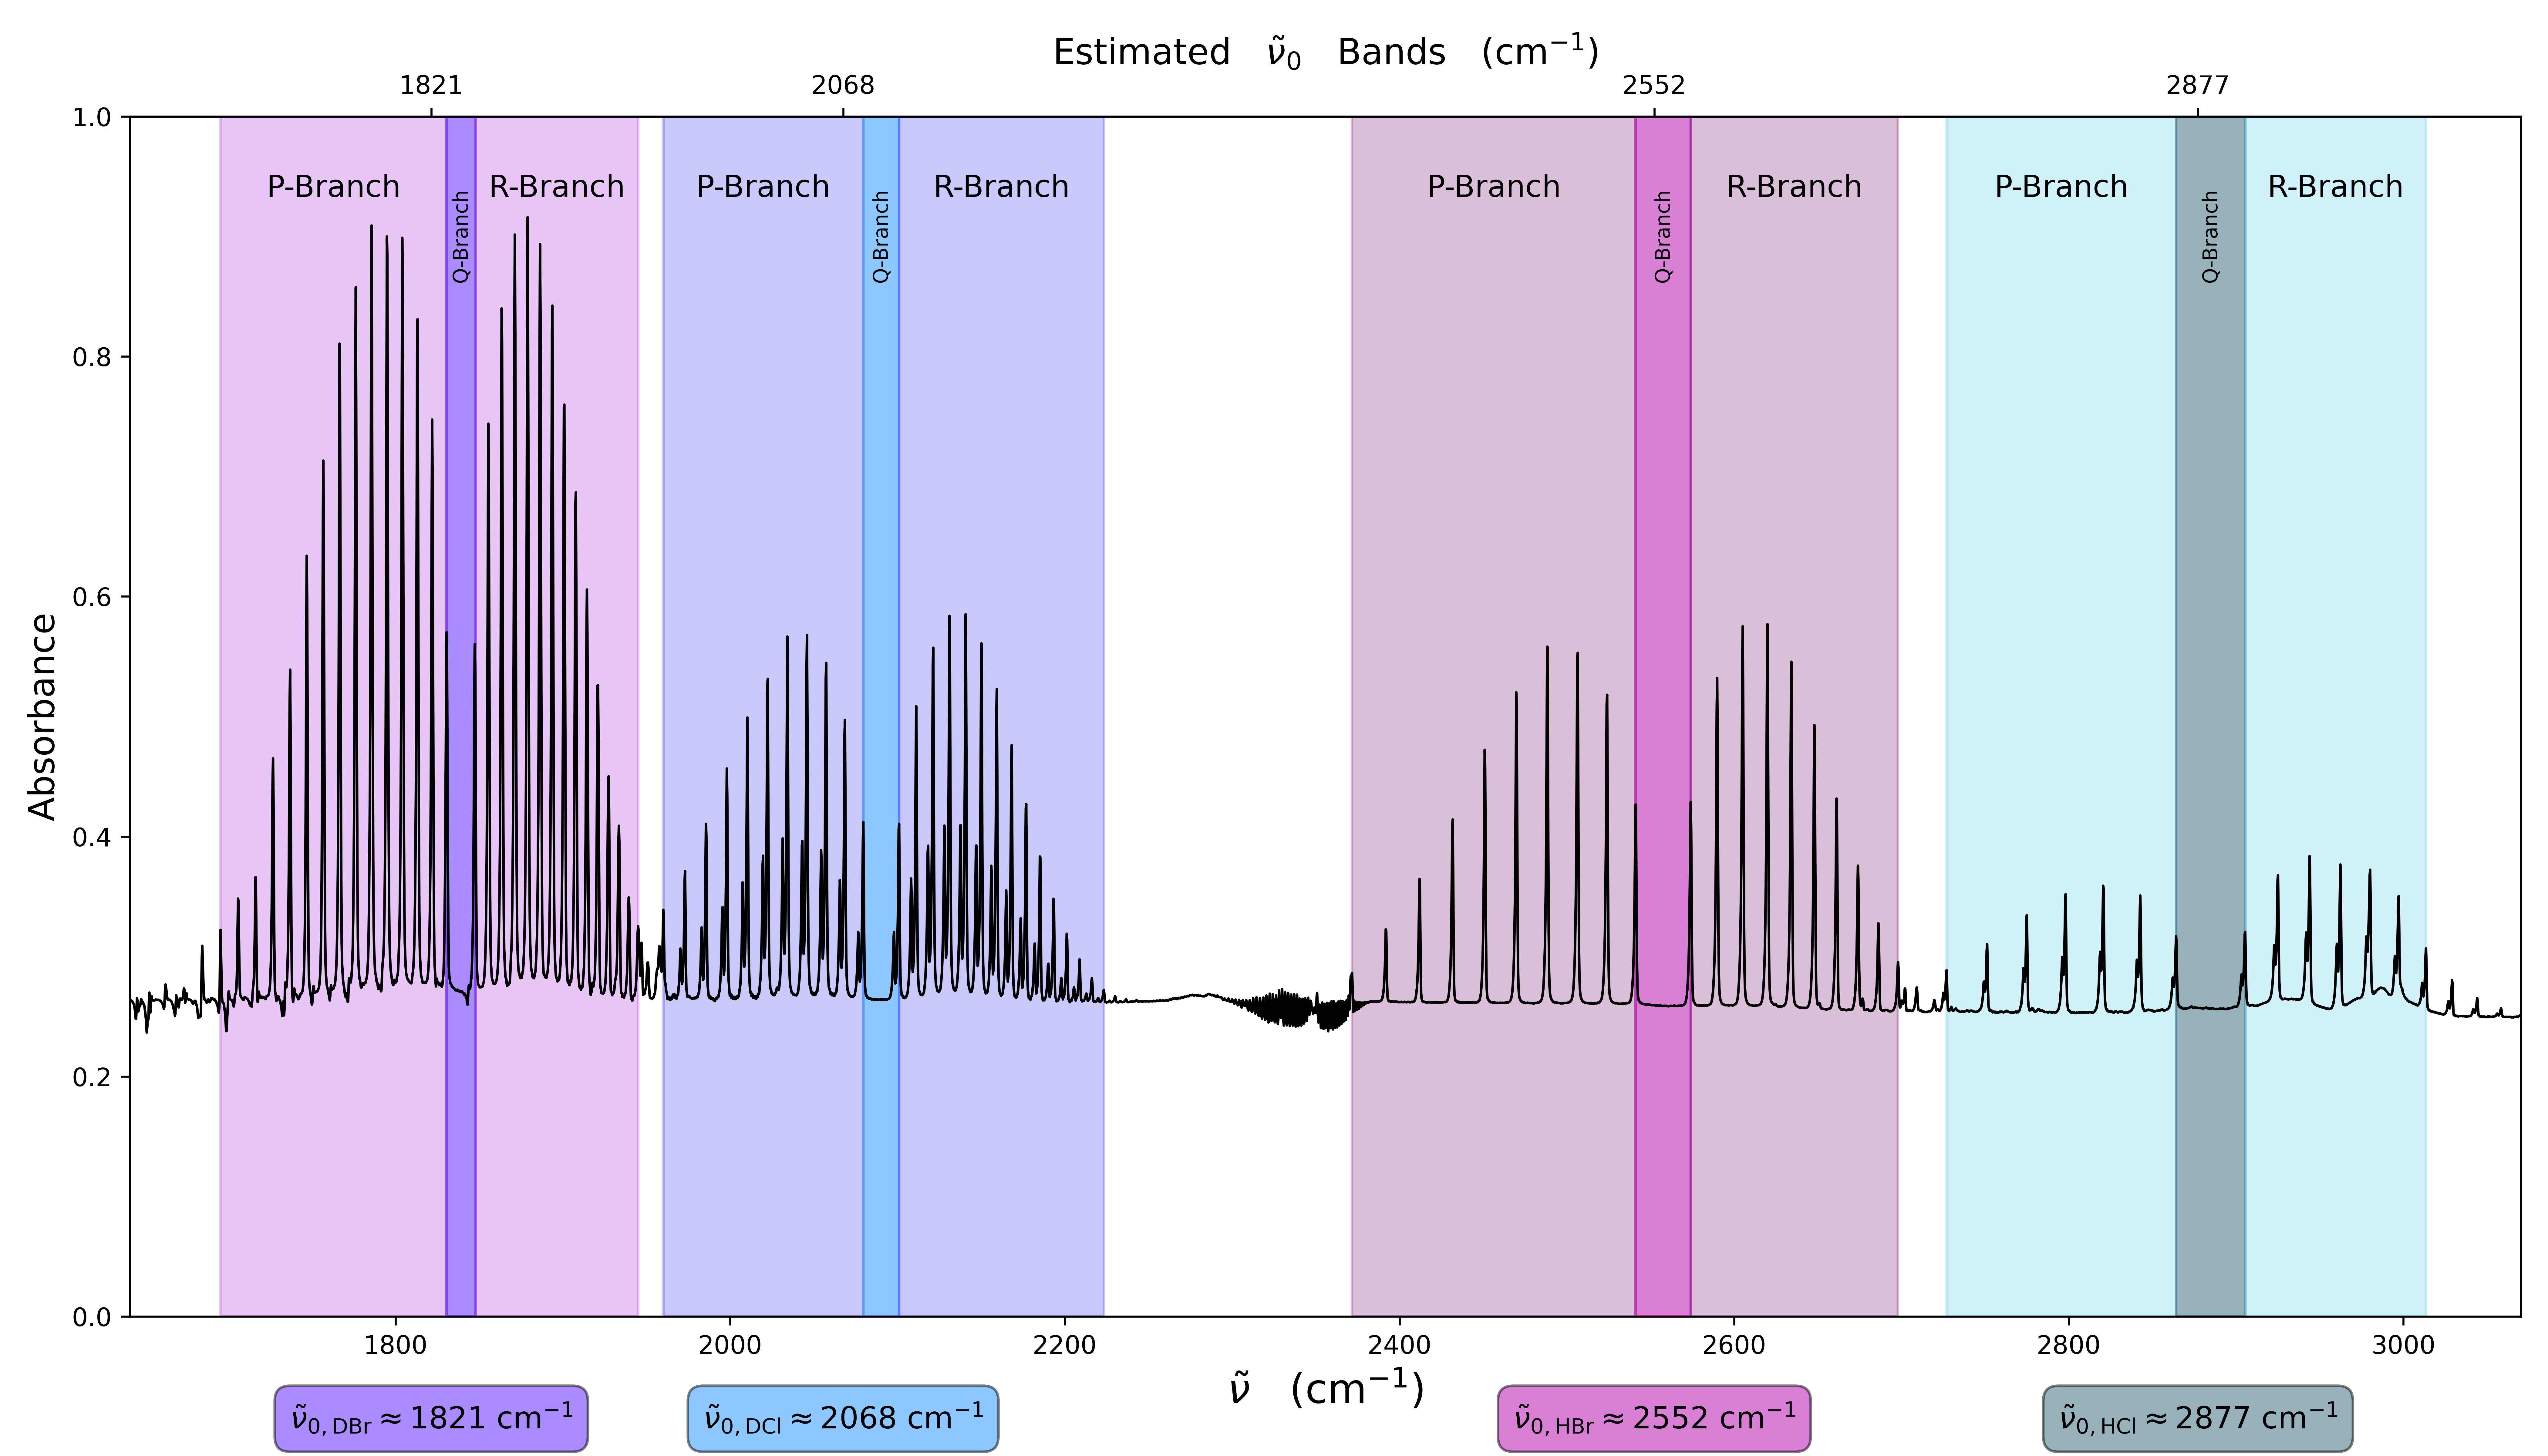
\includegraphics{example-analysis/rovib-spectra.png}
    \end{adjustbox}
    \caption{
        \emph{Species A: HCl, Species B: HBr, Species C: DCl, Species D: DBr}
    }
    \label{fig:spectra}
\end{sidewaysfigure}

\begin{figure}[hbtp]
    ~\usesubsection{Fundamental Frequency}
    The fundamental frequency, \(f_0\), for DBr is given by:
    \begin{align*}
        f_{0, DBr} &= \left(
            \frac{1}{2\pi}
        \right) \sqrt{\frac{k}{\mu_{DBr}}} \\
        &=\left(
            \frac{1}{2\pi}
        \right) \sqrt{\frac{384\,\mathrm{N/m}}{\left(79.9040\,\mathrm{amu}\right)\left(2.0141\,\mathrm{amu}\right)} \times \left(79.9040\,\mathrm{amu} + 2.0141\,\mathrm{amu}\right)} \\
        &= 5.46042386 \times 10^{13}\,\mathrm{Hz} \\
        &\mathbf{\approx 54.6\, THz = 1821\, cm^{-1}}
    \end{align*}
    ~\usesubsection{Peak Splitting}
    \par \indent The energy for the \(n^{th}\) vibrational mode is given by \(  E\left(v \right) = hf_{0}\left(n + \frac{1}{2}\right)\)where \(n = 0,1,2, 3, \cdots\) is the vibrational quantum  number
    and \(
        f_{0} = \frac{1}{2\pi}\sqrt{\frac{k}{\mu}}
        \) 
    is the fundamental vibrational frequency. The energy for the \(J^{th}\) rotational mode is given by \(
    E\left(J\right) = hcBJ\left(J + 1\right)
    \) where \(J=0,1,2,3,\cdots\) is the quantum rotational number, \(
    B = \frac{h}{8\pi^{2}cI}
    \) is the rotational constant, and \(
    I = \mu r^2_{e}
    \) is the moment of inertia. Under the Born-Oppenheimer approximation, the wavefunctions of the nucleus and electrons are considered distinct. This is due to the electrons being substantially smaller in mass than the nucleus (and therefore having a substantially higher angular frequency) which means we can more or less assume the nucleus is stationary with respect to its electrons. Therefore, we assume \emph{changes} in electron energy are only from electronic, vibrational, and rotational factors. A very simple model of simple diatomic molecules may be constructed where the total change in observed energy at a fixed electronic energy level is the sum of the vibrational and rotational energies. Since both the vibrational and rotational energies are dependent on the reduced mass of the system, \(
    \mu = \frac{m_1 m_2}{m_1 + m_2}
    \), the overall energy of a transition will be dependent on \(\mu\). 
    \\
    \par The transitions in the spectrum for HCl and DCl show doublets, indicating two different energies 
    are associated for the HCl and DCl rotational 
    transitions. This can be explained when we consider the two most common chlorine isotopes, \(\prescript{35}{}{Cl}\) 
    and \(\prescript{37}{}{Cl}\) with relative abundances of 
        \(\sim\)75\% and \(\sim\)25\% respectively
    (matching the observed splitting ratio of 3:1).
    The two most common isotopes of bromine are  \(\prescript{79}{}{Br}\) 
    and \(\prescript{81}{}{Br}\) (
        \(\sim\)51\% and \(\sim\)49\% respectively
    ) which leads to the assumption that the bromine spectra would split at a 1:1 ratio. However, we do not observe any splitting in the bromine lines. 
    \\
    \par\indent We can explain this by looking at the relative difference in \(\mu\) between the isotopes of the species.  
    The reduced masses for \(H\prescript{35}{}{Cl}\),
    \(H\prescript{79}{}{Br}\), \(D\prescript{35}{}{Cl}\), and \(D\prescript{79}{}{Br}\) are \(\mu_{H\prescript{35}{}{Cl}}\approx 0.9797\hspace*{2pt}amu,
    \mu_{H\prescript{79}{}{Br}} \approx 0.9952\hspace*{2pt}amu, 
    \mu_{D\prescript{35}{}{Cl}} \approx 1.9010\hspace*{2pt}amu,
    \quad \text{and} \quad
    \mu_{D\prescript{79}{}{Br}} \approx 1.9639\hspace*{2pt}amu
    \). The reduce masses for \(H\prescript{37}{}{Cl}\),
    \(H\prescript{81}{}{Br}\), \(D\prescript{37}{}{Cl}\), and \(D\prescript{81}{}{Br}\) are \(
        \mu_{H\prescript{37}{}{Cl}} \approx 0.9812\hspace*{2pt}amu,
        \mu_{H\prescript{81}{}{Br}} \approx 0.9955\hspace*{2pt}amu,
        \mu_{D\prescript{37}{}{Cl}} \approx 1.9099\hspace*{2pt}amu,
        \quad \text{and} \quad
        \mu_{D\prescript{81}{}{Br}} \approx 1.9651\hspace*{2pt}amu
    \). 
    \\
    \par \indent When compared, we see that the reduced masses of 
    \(H\prescript{35}{}{Cl}\) is \(\sim 0.15\%\) smaller than \(H\prescript{37}{}{Cl}\), 
    and that of  \(D\prescript{35}{}{Cl}\) is 
    and \(D\prescript{37}{}{Cl}\). On the other hand, the reduced 
    mass of \(H\prescript{79}{}{Br}\) is only \(\sim 0.030\%\) 
    smaller than \(H\prescript{81}{}{Br}\), whereas
    that of \(D\prescript{79}{}{Br}\) is only \(\sim 0.061\%\) smaller
    than the reduced mass of \(D\prescript{81}{}{Br}\). This suggests that splitting exists in bromine, but because the
    relative change in mass is so small the resulting peaks are too close together to resolve, whereas in chlorine the 
    difference is large enough to result in differentiable 
    bands leading to 
    the splitting pattern in its spectra. 
\end{figure}
    


% DBr Table
\begin{figure}[htbp]
    ~\usesubsection{Rotational Transitions}
    \centering\small
    % DBr (Top Left)
    \begin{minipage}[t]{0.48\textwidth}
        \centering
        \captionof{table}{Rotational Transitions for DBr}
        \begin{tabular}{|l|c|c|c|c|}
        \hline
        \textbf{Branch} & \(\mathbf{\tilde{\mathbf{\nu}}} \quad \left(cm^{-1}\right)\) 
        & \textbf{Abs.} & \(\mathbf{J_i}\) & \(\mathbf{J_f}\) \\ \hline
        P-Branch & 1695.48047 & 0.49287 & 15 & 14 \\ 
        P-Branch & 1705.93066 & 0.54563 & 14 & 13 \\ 
        P-Branch & 1716.38086 & 0.57693 & 13 & 12 \\ 
        P-Branch & 1726.83105 & 0.57522 & 12 & 11 \\ 
        P-Branch & 1737.02636 & 0.53206 & 11 & 10 \\ 
        P-Branch & 1746.96679 & 0.42879 & 10 & 9 \\ 
        P-Branch & 1756.90722 & 0.33888 & 9 & 8 \\ 
        P-Branch & 1766.59277 & 0.37125 & 8 & 7 \\ 
        P-Branch & 1776.27832 & 0.41061 & 7 & 6 \\ 
        P-Branch & 1785.70898 & 0.45668 & 6 & 5 \\ 
        P-Branch & 1794.88476 & 0.4991 & 5 & 4 \\ 
        P-Branch & 1804.06054 & 0.53141 & 4 & 3 \\ 
        P-Branch & 1813.23632 & 0.56661 & 3 & 2 \\ 
        P-Branch & 1821.90234 & 0.56802 & 2 & 1 \\ 
        P-Branch & 1830.56836 & 0.54466 & 1 & 0 \\ 
        \hhline{|=====|}
        R-Branch & 1847.90039 & 0.4971 & 0 & 1 \\ 
        R-Branch & 1855.54687 & 0.41204 & 1 & 2 \\ 
        R-Branch & 1863.44824 & 0.27222 & 2 & 3 \\ 
        R-Branch & 1871.34961 & 0.28195 & 3 & 4 \\ 
        R-Branch & 1878.99609 & 0.29763 & 4 & 5 \\ 
        R-Branch & 1886.38769 & 0.31897 & 5 & 6 \\ 
        R-Branch & 1893.77929 & 0.34817 & 6 & 7 \\ 
        R-Branch & 1900.91601 & 0.38331 & 7 & 8 \\ 
        R-Branch & 1907.79785 & 0.42709 & 8 & 9 \\ 
        R-Branch & 1914.4248 & 0.47608 & 9 & 10 \\ 
        R-Branch & 1921.05175 & 0.52298 & 10 & 11 \\ 
        R-Branch & 1927.42382 & 0.56092 & 11 & 12 \\ 
        R-Branch & 1933.54101 & 0.58517 & 12 & 13 \\ 
        R-Branch & 1939.40332 & 0.58385 & 13 & 14 \\ 
        R-Branch & 1945.01074 & 0.5573 & 14 & 15 \\ \hline
        \end{tabular}
        \label{tab:dbr}
    \end{minipage}
    \vspace{2em}
    \hfill
    % DCl (Top Right)
    \begin{minipage}[t]{0.48\textwidth}
        \centering
        \captionof{table}{Rotational Transitions for DCl}
        \begin{tabular}{|l|c|c|c|c|}
        \hline
        \textbf{Branch} & \(\mathbf{\tilde{\nu}} \quad \left(cm^{-1}\right)\) 
        & \textbf{Abs.} & \(\mathbf{J_i}\) & \(\mathbf{J_f}\) \\ \hline
        P-Branch & 1960.04882 & 0.41422 & 11 & 10 \\ 
        P-Branch & 1973.04785 & 0.47226 & 10 & 9 \\ 
        P-Branch & 1985.53711 & 0.52025 & 9 & 8 \\ 
        P-Branch & 1998.02636 & 0.55819 & 8 & 7 \\ 
        P-Branch & 2010.26074 & 0.55305 & 7 & 6 \\ 
        P-Branch & 2022.49511 & 0.51809 & 6 & 5 \\ 
        P-Branch & 2034.21972 & 0.42659 & 5 & 4 \\ 
        P-Branch & 2045.94433 & 0.29537 & 4 & 3 \\ 
        P-Branch & 2057.41406 & 0.32779 & 3 & 2 \\ 
        P-Branch & 2068.6289 & 0.37569 & 2 & 1 \\ 
        P-Branch & 2079.58886 & 0.43162 & 1 & 0 \\
        \hhline{|=====|}
        R-Branch & 2100.99902 & 0.50871 & 0 & 1 \\
        R-Branch & 2111.19433 & 0.4106 & 1 & 2 \\ 
        R-Branch & 2121.38965 & 0.32223 & 2 & 3 \\ 
        R-Branch & 2131.07519 & 0.34832 & 3 & 4 \\ 
        R-Branch & 2140.76074 & 0.36626 & 4 & 5 \\ 
        R-Branch & 2150.1914 & 0.46512 & 5 & 6 \\ 
        R-Branch & 2159.36718 & 0.53905 & 6 & 7 \\ 
        R-Branch & 2168.28808 & 0.63392 & 7 & 8 \\ 
        R-Branch & 2176.9541 & 0.71318 & 8 & 9 \\ 
        R-Branch & 2185.11035 & 0.81072 & 9 & 10 \\ 
        R-Branch & 2193.2666 & 0.85761 & 10 & 11 \\ 
        R-Branch & 2201.16797 & 0.9091 & 11 & 12 \\ 
        R-Branch & 2208.81445 & 0.89994 & 12 & 13 \\ 
        R-Branch & 2216.20605 & 0.89895 & 13 & 14 \\ 
        R-Branch & 2223.34277 & 0.83108 & 14 & 15 \\ \hline
        \end{tabular}
        \label{tab:dcl}
    \end{minipage}
    \vspace{4mm}
    % HBr (Bottom Left)
    \begin{minipage}[t]{0.48\textwidth}
        \centering
        \captionof{table}{Rotational Transitions for HBr}
        \begin{tabular}{|l|c|c|c|c|}
        \hline
        \textbf{Branch} & \(\mathbf{\tilde{\nu}} \quad \left(cm^{-1}\right)\) 
        & \textbf{Abs.} & \(\mathbf{J_i}\) & \(\mathbf{J_f}\) \\ \hline
        P-Branch & 2371.68457 & 0.30671 & 10 & 9 \\ 
        P-Branch & 2391.82031 & 0.35042 & 9 & 8 \\ 
        P-Branch & 2411.95605 & 0.37233 & 8 & 7 \\ 
        P-Branch & 2431.83691 & 0.37666 & 7 & 6 \\ 
        P-Branch & 2450.95312 & 0.38368 & 6 & 5 \\ 
        P-Branch & 2469.81445 & 0.36769 & 5 & 4 \\ 
        P-Branch & 2488.4209 & 0.32051 & 4 & 3 \\ 
        P-Branch & 2506.51757 & 0.28632 & 3 & 2 \\ 
        P-Branch & 2524.10449 & 0.32267 & 2 & 1 \\ 
        P-Branch & 2541.18164 & 0.36468 & 1 & 0 \\ 
        \hhline{|=====|}
        R-Branch & 2574.06152 & 0.74744 & 0 & 1 \\ 
        R-Branch & 2589.86425 & 0.57012 & 1 & 2 \\ 
        R-Branch & 2605.15722 & 0.32528 & 2 & 3 \\ 
        R-Branch & 2619.94043 & 0.34923 & 3 & 4 \\ 
        R-Branch & 2634.21386 & 0.40899 & 4 & 5 \\ 
        R-Branch & 2647.97754 & 0.4501 & 5 & 6 \\ 
        R-Branch & 2661.23144 & 0.52606 & 6 & 7 \\ 
        R-Branch & 2673.97558 & 0.60582 & 7 & 8 \\ 
        R-Branch & 2686.20996 & 0.68695 & 8 & 9 \\ 
        R-Branch & 2697.93457 & 0.75986 & 9 & 10 \\ \hline
        \end{tabular}
        \label{tab:hbr}
    \end{minipage}
    \hfill
    % HCl (Bottom Right)
    \begin{minipage}[t]{0.48\textwidth}
        \centering
        \captionof{table}{Rotational Transitions for HCl}
        \begin{tabular}{|l|c|c|c|c|}
        \hline
        \textbf{Branch} & \(\mathbf{\tilde{\nu}} \quad \left(cm^{-1}\right)\) 
        & \textbf{Abs.} & \(\mathbf{J_i}\) & \(\mathbf{J_f}\) \\ \hline
        P-Branch & 2726.99121 & 0.28859 & 7 & 6 \\ 
        P-Branch & 2751.20507 & 0.31044 & 6 & 5 \\ 
        P-Branch & 2774.90918 & 0.33444 & 5 & 4 \\ 
        P-Branch & 2798.10351 & 0.35194 & 4 & 3 \\ 
        P-Branch & 2820.5332 & 0.35902 & 3 & 2 \\ 
        P-Branch & 2842.708 & 0.35084 & 2 & 1 \\ 
        P-Branch & 2864.11816 & 0.31705 & 1 & 0 \\ 
        \hhline{|=====|}
        R-Branch & 2905.40918 & 0.84236 & 0 & 1 \\ 
        R-Branch & 2925.03515 & 0.89374 & 1 & 2 \\ 
        R-Branch & 2943.89648 & 0.916 & 2 & 3 \\ 
        R-Branch & 2962.24804 & 0.90156 & 3 & 4 \\ 
        R-Branch & 2980.08984 & 0.84005 & 4 & 5 \\ 
        R-Branch & 2997.16699 & 0.74405 & 5 & 6 \\ 
        R-Branch & 3013.47949 & 0.46666 & 6 & 7 \\ \hline
        \end{tabular}
        \label{tab:hcl}
    \end{minipage}
\end{figure}

\begin{figure}[hbtp]
    ~\usesection{Model Fits}
    \vspace{-2em}
    ~\usesubsection{DBr}
    {\small
        \verbatiminput{example-analysis/dbr.txt}
    }
\end{figure}
\begin{figure}[hbtp]
    ~\usesubsection{DCl}
    {\small
        \verbatiminput{example-analysis/dcl.txt}
    }
\end{figure}
\begin{figure}[hbtp]
    ~\usesubsection{HBr}
    {\small
        \verbatiminput{example-analysis/hbr.txt}
    }
\end{figure}
\begin{figure}[hbtp]
    ~\usesubsection{HCl}
    {\small
        \verbatiminput{example-analysis/hcl.txt}
    }
\end{figure}

\newpage
\begin{figure}[hbtp]
    ~\usesection{Zero Order Model}
    \centering
    \begin{minipage}[t]{\textwidth}
        \centering
        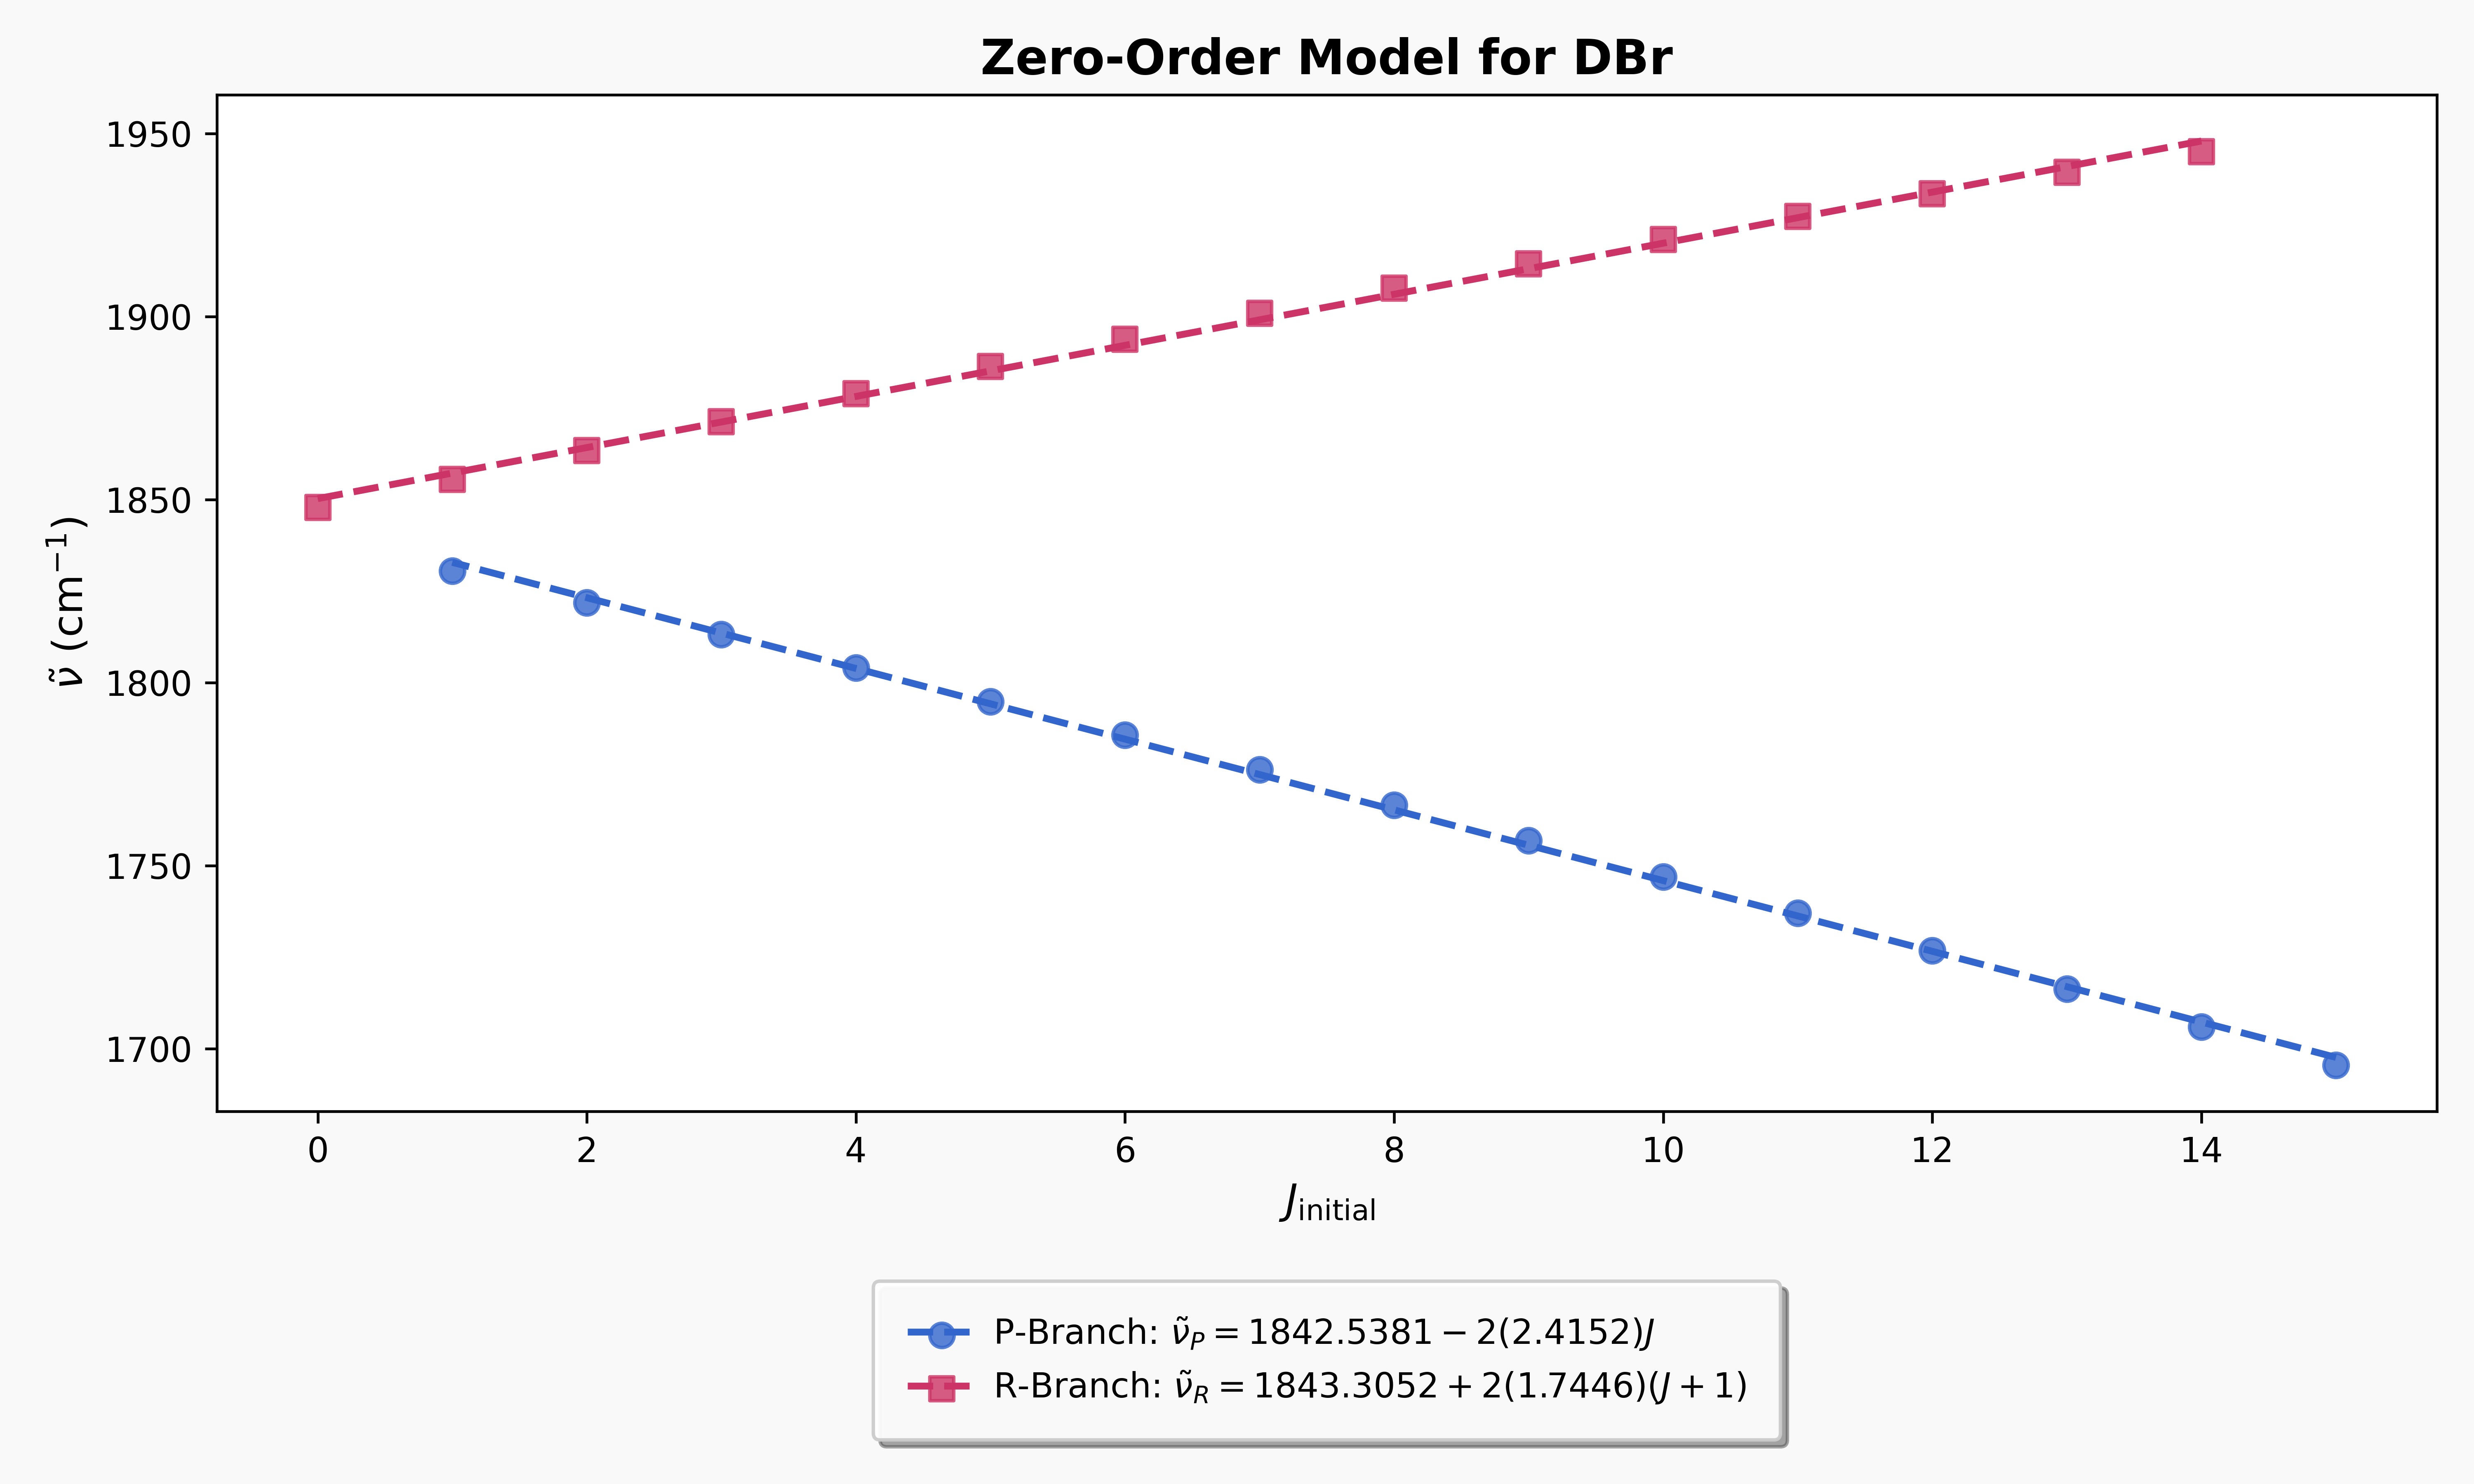
\includegraphics[width=\linewidth]{example-analysis/dbr-zero-order-fit.png}
        \caption*{\mbox{}}
    \end{minipage}
    \begin{minipage}[t]{\textwidth}
            \centering
            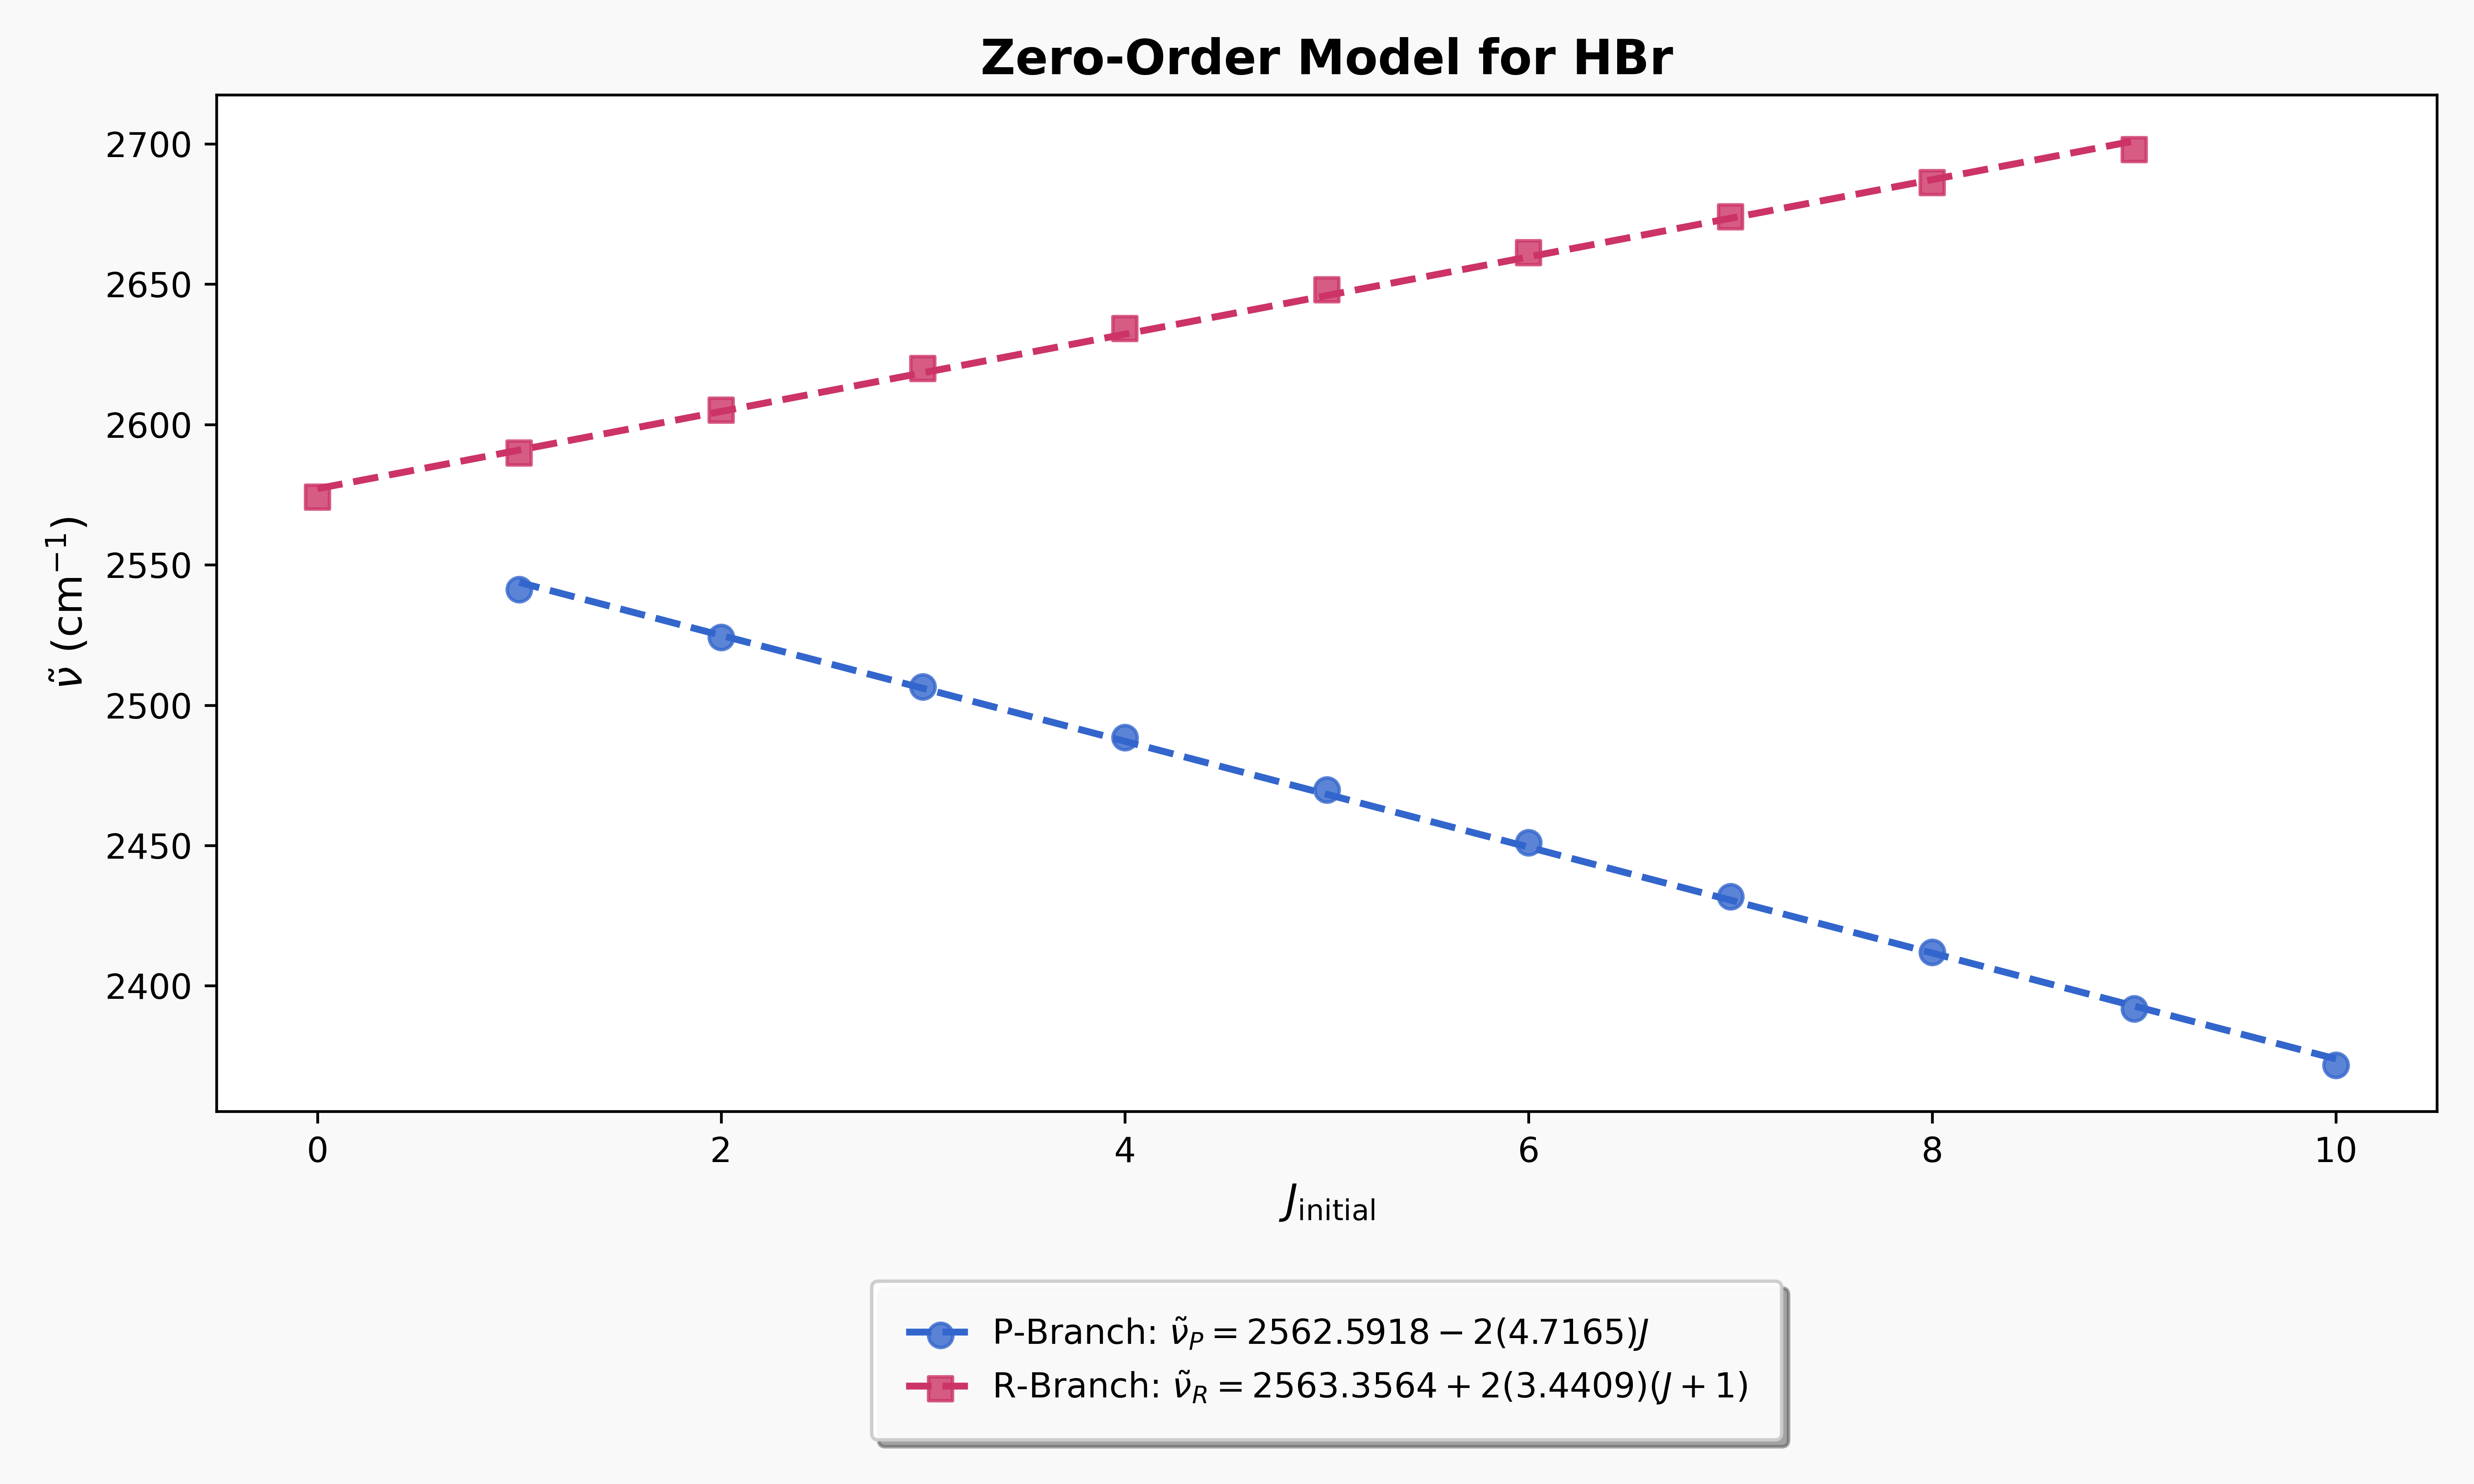
\includegraphics[width=\linewidth]{example-analysis/hbr-zero-order-fit.png}
        \end{minipage}
\end{figure}
\begin{figure}[htbp]
    \begin{minipage}[t]{\textwidth}
        \centering
        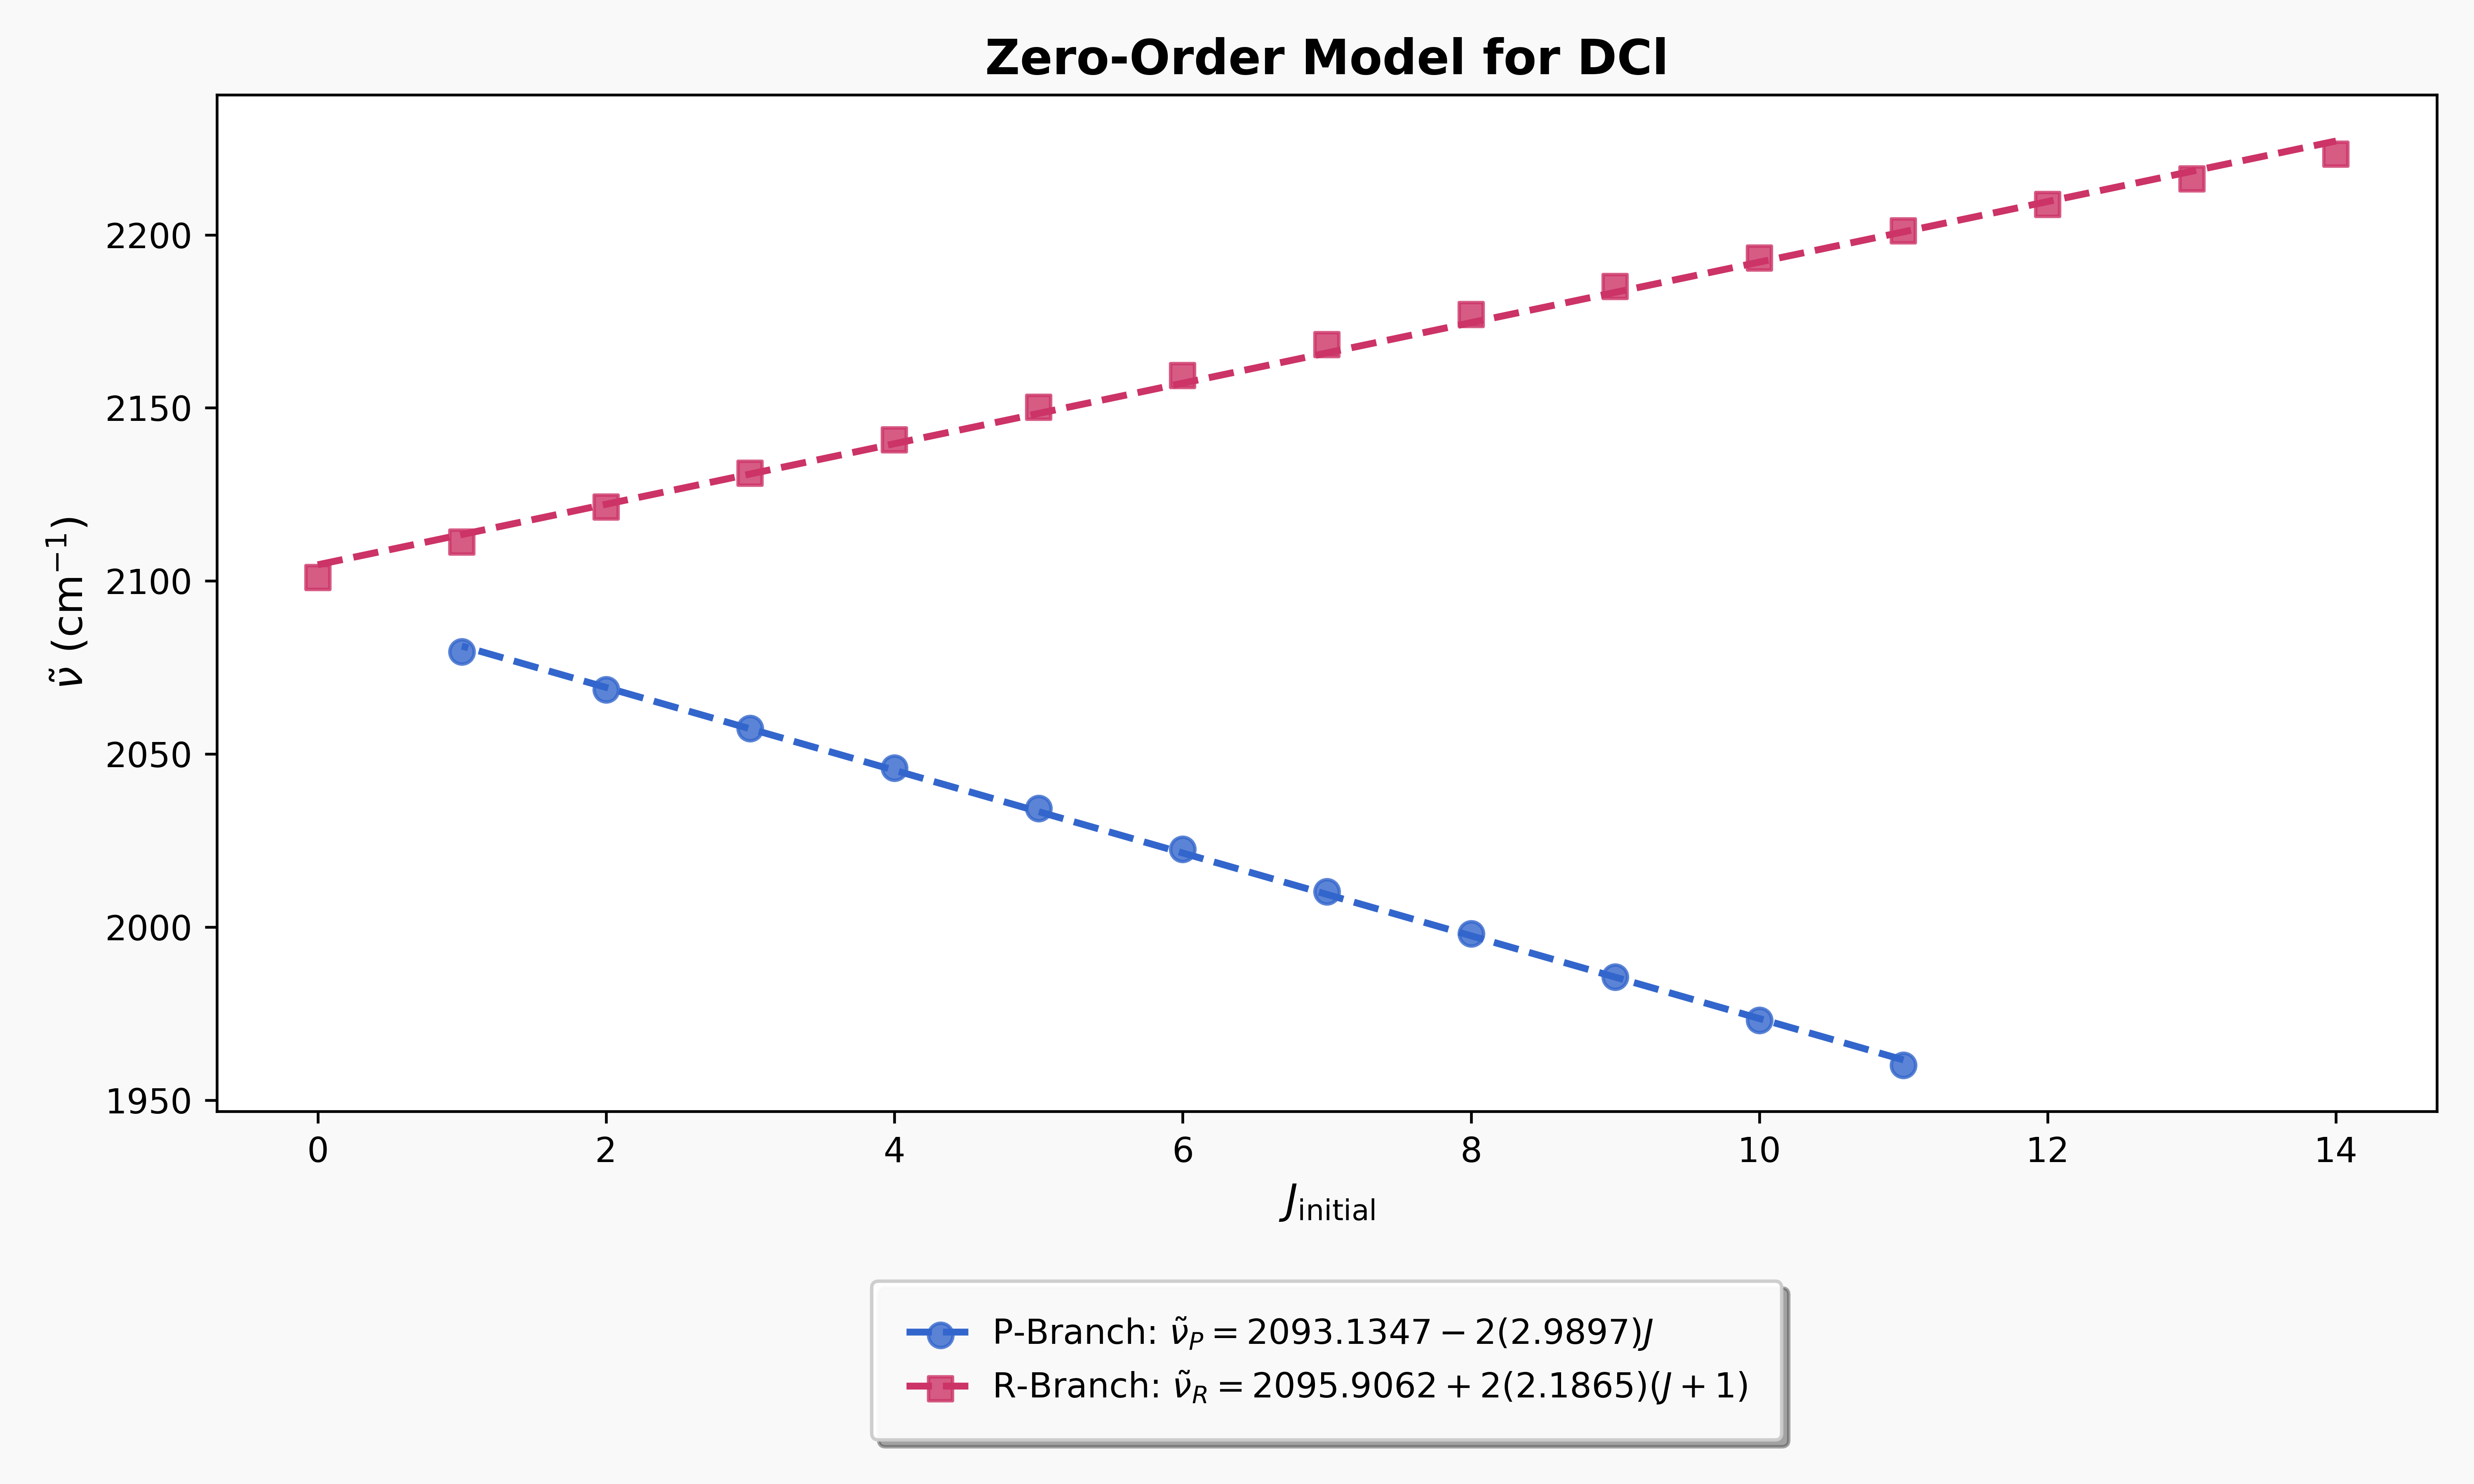
\includegraphics[width=\linewidth]{example-analysis/dcl-zero-order-fit.png}
    \end{minipage}
\caption*{\mbox{}}
\begin{minipage}[t]{\textwidth}
        \centering
        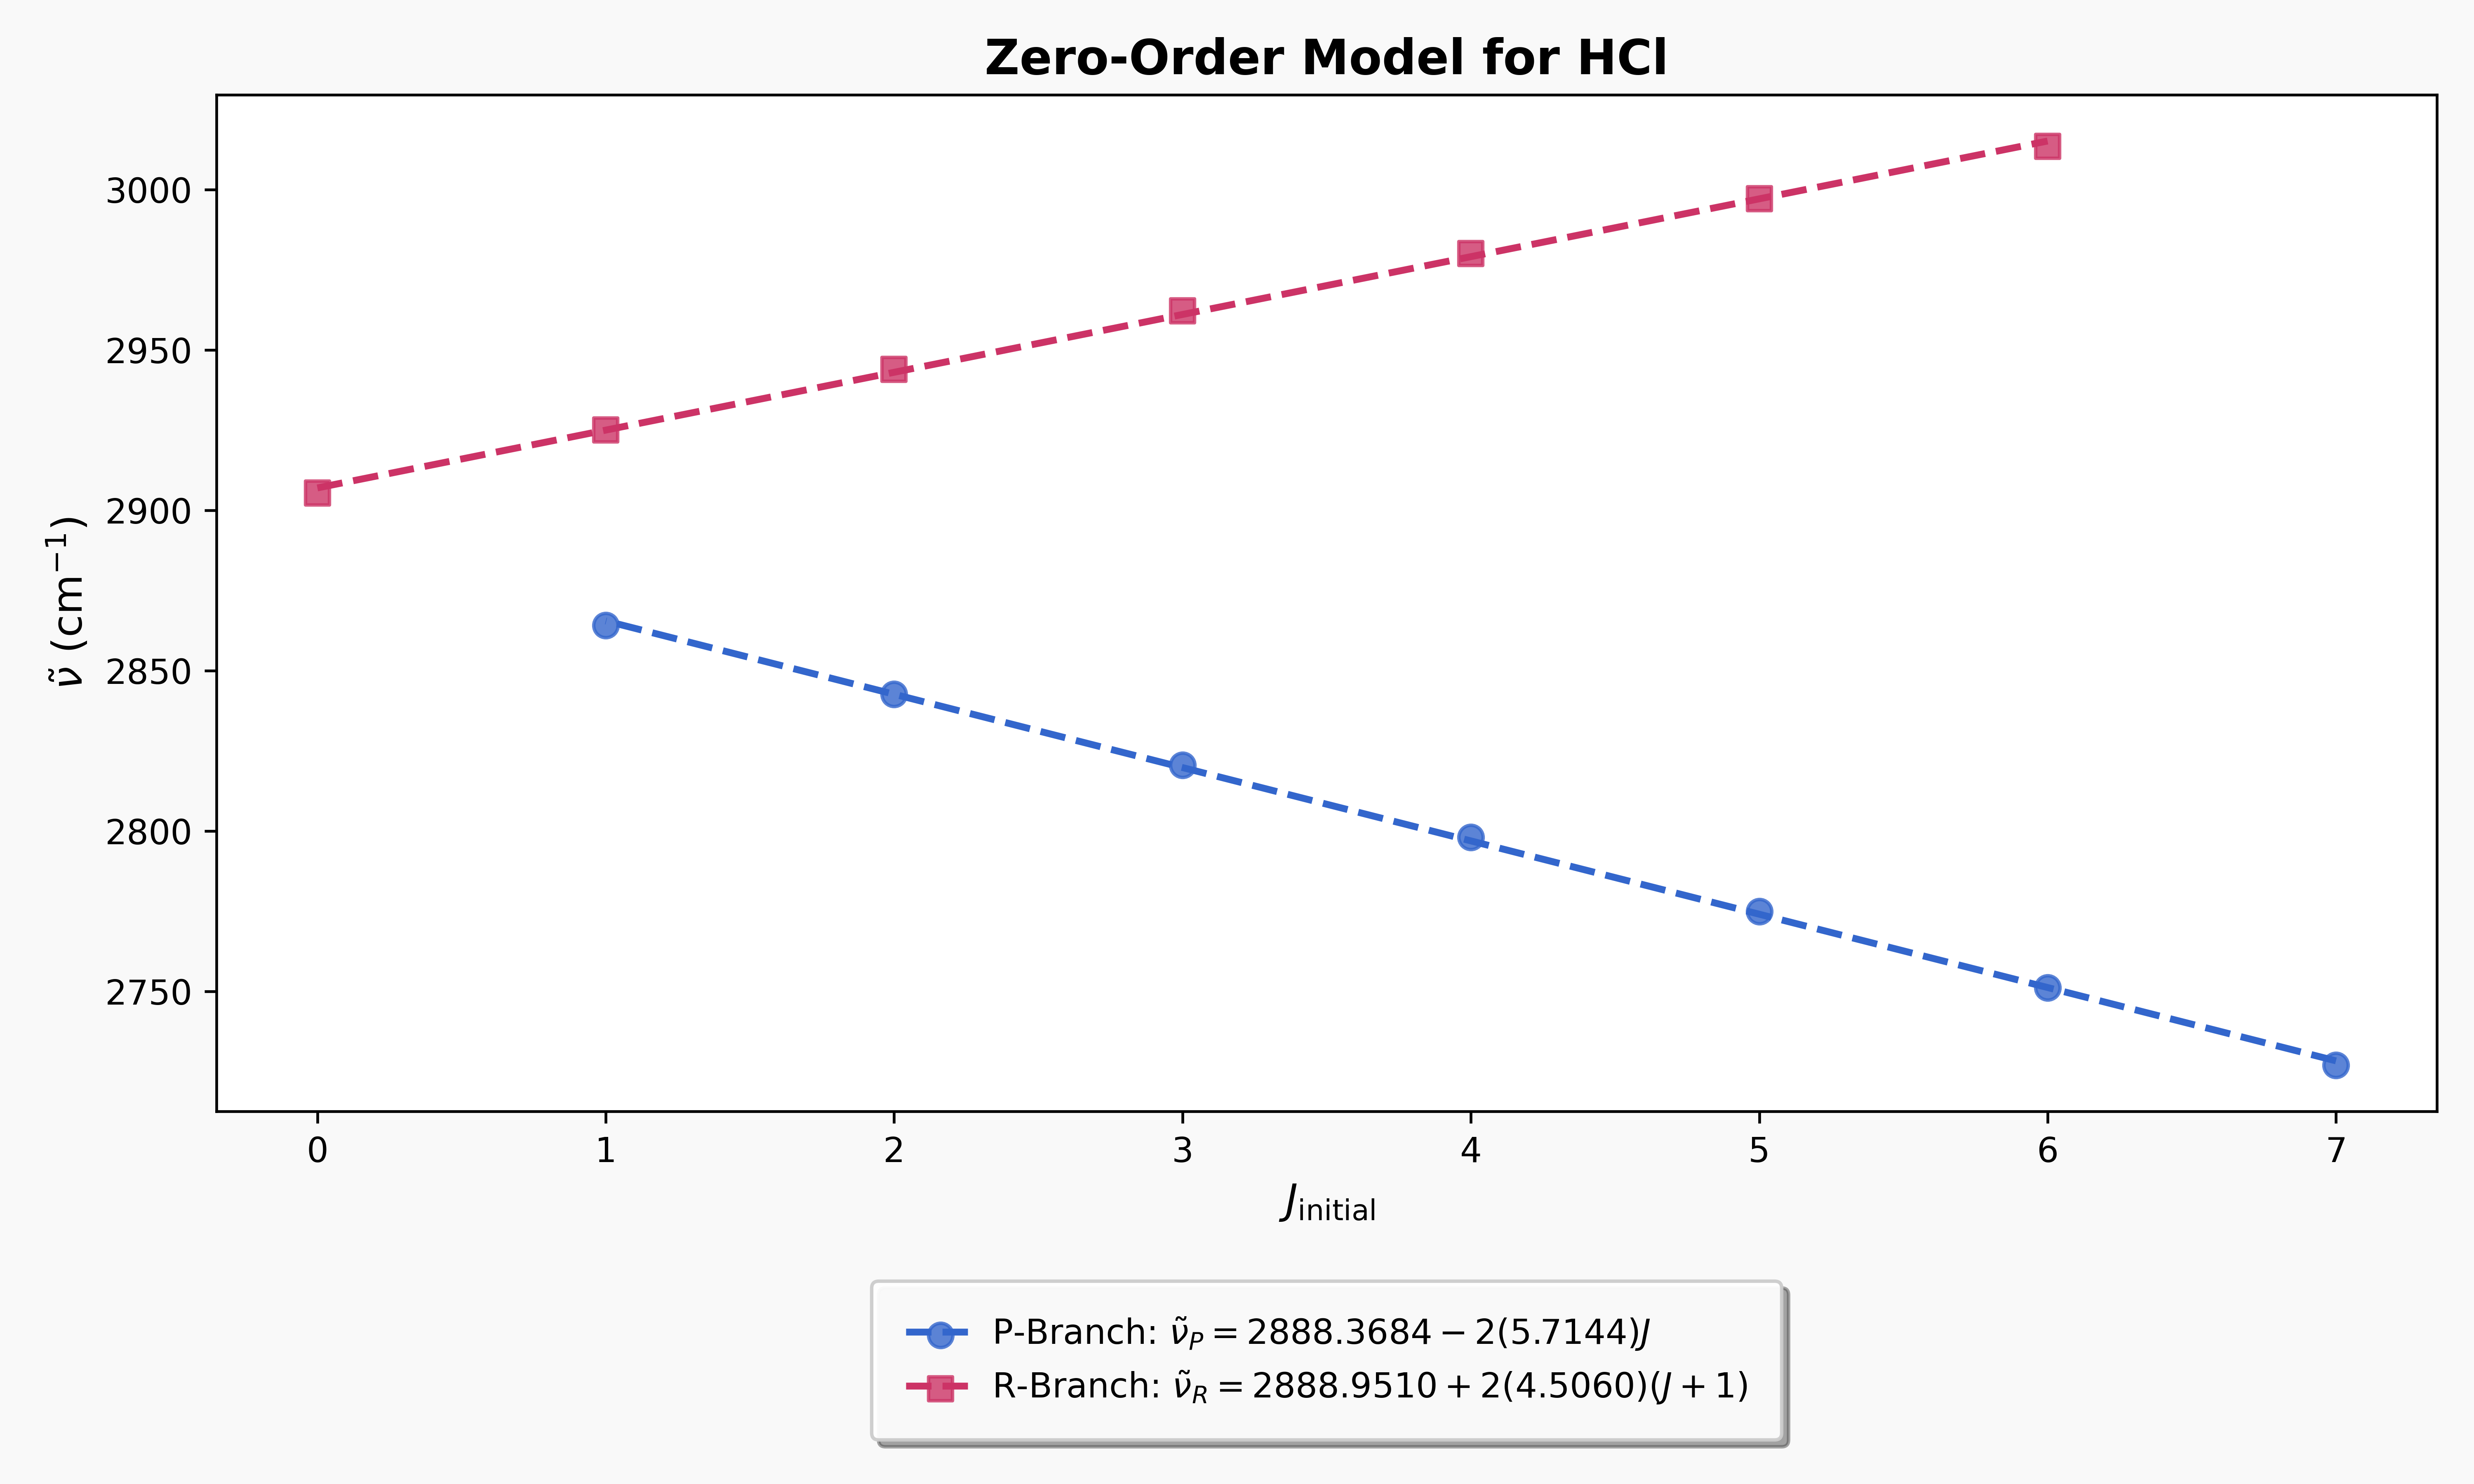
\includegraphics[width=\linewidth]{example-analysis/hcl-zero-order-fit.png}
    \end{minipage}
\end{figure}

\begin{figure}[htbp]
    ~\usesubsection{Background}
    The energy for the zero model approximation is given by:
    \begin{align*}
        E_{0} &= h f_{0} \left(
            n + \frac{1}{2}
        \right) + hc BJ\left(J+1\right)
    \end{align*}
    The zero order approximation assumes the diatomic molecule
    consists of two distinct systems: a simple harmonic oscillator
    (SHO) representing the vibrational energy, and a rigid rotator
    (RR) representing the rotational energy. 
    The peak in a rovib spectra is therefore the sum of the 
    change in vibrational energy and the change in rotational
    energy. The vibrational transition is from \(n=0\) to \(n=1\) (\(n\rightarrow n+1\)),
    where \( n=0\) is at the fundamental vibrational frequency \(f_{0}\).
    The energy from this transition is given by
    \begin{align*}
        \Delta E_{n} &= E_{n}\left(
            n + 1
        \right) - E_{n}\left(
            n
        \right) \\
        &= hf_{0} \left(
            n+1+\frac{1}{2}
            \right) 
            - hf_{0} \left(
                n + \frac{1}{2}
            \right) \\
        &= hf_{0}\left[
            \left(
                n + \frac{3}{2}
            \right)
            - \left(
                n + \frac{1}{2}
            \right)
        \right] \\
        &= hf_{0} \\
    \end{align*}
    By the selection rules for rotational transitions, 
    \(\Delta J = \pm 1\), leading to the two observed branches
    corresponding to  \(J \rightarrow J - 1\) (the `P-Branch') 
    and  \(J \rightarrow J + 1\) (the `R-Branch').
    ~\usesubsection{P-Branch Derivations}
    The change in energy for the P-Branch is given by 
    \begin{align*}
        \Delta E_{J, P} &= E_{J}\left(J-1\right) - E_{J}\left(J\right) \\
        &= h c B \left(
            J-1
            \right)\left(
            J-1+1
            \right) - h c B \left(J\left(J+1\right)\right) \\
        &= h c B \left[J
            \left(J - 1\right)- J\left(J + 1 \right)
        \right] \\
        &= h c B \left(-2J\right) \\
        &= -hc\left(2BJ\right)\\
    \end{align*}
    And the total change in energy for a given transition
    \begin{align*}
        \Delta E_{0, P} &= \Delta E_{n} + \Delta E_{J, P} \\
        \Delta E_{0, P} &= hf_{0}
        - h c\left(2BJ \right) \\
        \frac{\Delta E_{0, P}}{hc} &= 
        \frac{f_{0}}{c} - 2BJ\\
        \tilde{\nu}_{P} &= \tilde{\nu}_0 - 2BJ \quad  \\
    \end{align*}
\end{figure}
\begin{figure}[hbtp]
    ~\usesubsection{R-Branch Derivations}
    A similar approach can be used for the R-Branch to find the 
    energy of a specific transition
    \begin{align*}
    \Delta E_{J, R} &= E_{J}\left(J+1\right) -E_{J}\left(J\right) \\
        &= h c B \left(J+1\right)\left(J+1+1\right) - h c B \left(J\left(J+1\right)\right) \\
        &= h c B \left[
            \left(J + 1\right)\left(J + 2\right) - J\left(J + 1 \right)
        \right] \\
        &= h c B \left(2J + 2\right) \\
        &= h c\left(2B \right)\left(J + 1\right) \\
    \end{align*}
And now solving for the energy of the peak
\begin{align*}
    \Delta E_{0, R} &=  \Delta E_{n}
        + \Delta E_{J}\left(
            J
        \right)_{R} \\
        \Delta E_{0, R} &= hf_{0}
        + h c\left(2B \right)\left(J + 1\right) \\
        \frac{\Delta E_{0, R}}{hc} &= 
        \frac{f_{0}}{c} + 2B\left(J + 1\right) \\
        \tilde{\nu}_{R} &= \tilde{\nu}_0 + 
        2B\left(J + 1\right) \quad  \\
    \end{align*}
    ~\usesubsection{Fundamental Wavenumber}
The zero order fit assumes the  \(
\tilde{\nu} = \tilde{\nu}_{0} + 2B\left(J+1\right)
\) and for the P-branch we get \(
    \tilde{\nu} = \tilde{\nu}_{0} - 2BJ
\). After we perform a linear regression on the data for DBr, we get \(
\tilde{\nu}_{R} = 1843.3052 + 2\left(
    1.7446
\right) \left(
    J + 1
\right) \) and \(
    \tilde{\nu}_{P} = 1842.5381 - 2\left(2.4152\right)J
\).
The average value is  therefore
\begin{align*}
    \tilde{\nu}_{0} &= \frac{\tilde{\nu}_{R} + \tilde{\nu}_P}{2} \\
    &= \frac{1842.5381 + 1843.3052}{2} \\
    &\approx 1842.9217 \mathrm{cm}^{-1} \\
    SD &= \sqrt{
        \frac{
            \left(
                1842.5381 - 1842.9217
            \right)^2
        + \left(
            1843.3052 - 1842.9217
        \right)^2
        }{2}
    } \\
    &\approx 0.383550 \mathrm{cm}^{-1} \\
    SE &= \frac{SD}{\sqrt{2}} \\
    &= \frac{0.383550}{\sqrt{2}} \\
    & \approx 0.2712 \mathrm{cm}^{-1} \\
    \mathbf{\tilde{\nu}}_{0} &= \mathbf{
        \left(
            1842.9 \pm 0.2712
        \right) cm^{-1}
    } \\
\end{align*}
\end{figure}
\begin{figure}[hbtp]
    ~\usesubsection{Rotational Constant}
B represents the rotational constant, which is inversely proportional to the molecule's moment of inertia, 
mass, and equilibrium radius. It is directly related to the spacing of successive peaks and is therefore
proportional to the change in energy between transitions. Using DBr as the model, the derivation of B is
shown below.  
\begin{align*}
    B &= \frac{B_{R} + B_{P}}{2} \\
    &= \frac{1.7446 + 2.4152}{2} \\
    &= 2.0799 \mathrm{cm}^{-1} \\
    SD &= \sqrt{
        \frac{
            \left(
                1.7446 - 2.0799
            \right)^2
        + \left(
            2.4152 - 2.0799
        \right)^2
        }{2}
    } \\
    &= 0.3353 \mathrm{cm}^{-1} \\
    SE &= \frac{SD}{\sqrt{2}} \\
    &= \frac{0.3353}{\sqrt{2}} \\ 
    & \approx 0.2371 \mathrm{cm}^{-1} \\
    \mathbf{B} &= \mathbf{
        \left(
            2.0799 \pm 0.2371
        \right) cm^{-1}
    } \\
\end{align*}
~\usesubsection{Equilibrium Radius}    
The equation for the rotational constant is \(
    B = \frac{h}{8 \pi^2 c I} 
    \) where \( 
    I = \mu r_{e}^2
    \). Rearranging gives \(
    r_{e} = \sqrt{
        \frac{h}{8 \pi^2 c \mu  B}}
\). For the R-Branch, the calculated \(r_{e}\) is
\begin{align*}
    r_{e, R} &= \sqrt{
        \frac{h}{8 \pi^2 c \mu_{\text{\scriptsize DBr}}  B_{R}}} \\
    &= \sqrt{
    \frac{0.0399031221 \mathring{A}^2 \cdot \nicefrac{\mathrm{amu}}{\mathrm{fs}}}{
    \left(
        8 \pi^2
    \right)    
    \left(
        2.99792458\times 10^{3}\nicefrac{\mathring{A}}{\mathrm{fs}}
    \right) \left(
        1.9646 \cdot \mathrm{amu}
    \right)
    \left(
        1.7446 \times 10^{-8} \mathring{A}^{-1}
    \right) 
    }}\\
    &\approx 2.2178 \mathring{A} \\
\end{align*}
\end{figure}
\begin{figure}[hbtp]
    For the P-Branch, \(r_e\) is
    \begin{align*}
        r_{e, P} &= \sqrt{
        \frac{h}{8 \pi^2 c \mu_{\text{\scriptsize DBr}}  B_{P}}} \\
    &= \sqrt{
    \frac{0.0399031221 \mathring{A}^2 \cdot \nicefrac{\mathrm{amu}}{\mathrm{fs}}}{
    \left(
        8 \pi^2
    \right)    
    \left(
        2.99792458\times 10^{3}\nicefrac{\mathring{A}}{\mathrm{fs}}
    \right) \left(
        1.9646 \cdot \mathrm{amu}
    \right)
    \left(
        2.4152 \times 10^{-8} \mathring{A}^{-1}
    \right) 
    }}\\
    &\approx 1.8849 \mathring{A} \\
    \end{align*}
    The average value is  therefore
\begin{align*}
    r_{e} &= \frac{ r_{e, R} + r_{e, P}}{2} \\
    &= \frac{2.2178 + 1.8849}{2} \\
    &\approx 2.05135 \mathring{A} \\
    SD &= \sqrt{
        \frac{
            \left(
                2.2178 - 2.05135
            \right)^2
        + \left(
            1.8849 - 2.05135
        \right)^2
        }{2}
    } \\
    &\approx 0.16645 \mathring{A} \\
    SE &= \frac{SD}{\sqrt{2}} \\
    &= \frac{0.16645}{\sqrt{2}} \\
    & \approx 0.1177 \mathring{A} \\
    \mathbf{r_e} &= \mathbf{
        \left(
            2.0513 \pm 0.1177
        \right) \mathring{A}
    } \\
\end{align*}
    ~\usesubsection{Moment of Inertia}
    The moment of inertia for the P-branch is \(
    I_{P} \approx 6.9797 \mathrm{amu} \cdot \mathring{A}^2
    \) and for the R-Branch \(
    I_{R} \approx 9.6628 \mathrm{amu} \cdot \mathring{A}^2
    \). This gives an average of \(
    \mathbf{\left(
        8.3213 \pm 0.9486
    \right) amu \cdot \mathring{A}^2}
    \)
\end{figure}

\newpage
\begin{figure}[hbtp]
    ~\usesection{First Order Model}
    \centering
    \begin{minipage}[t]{\textwidth}
        \centering
        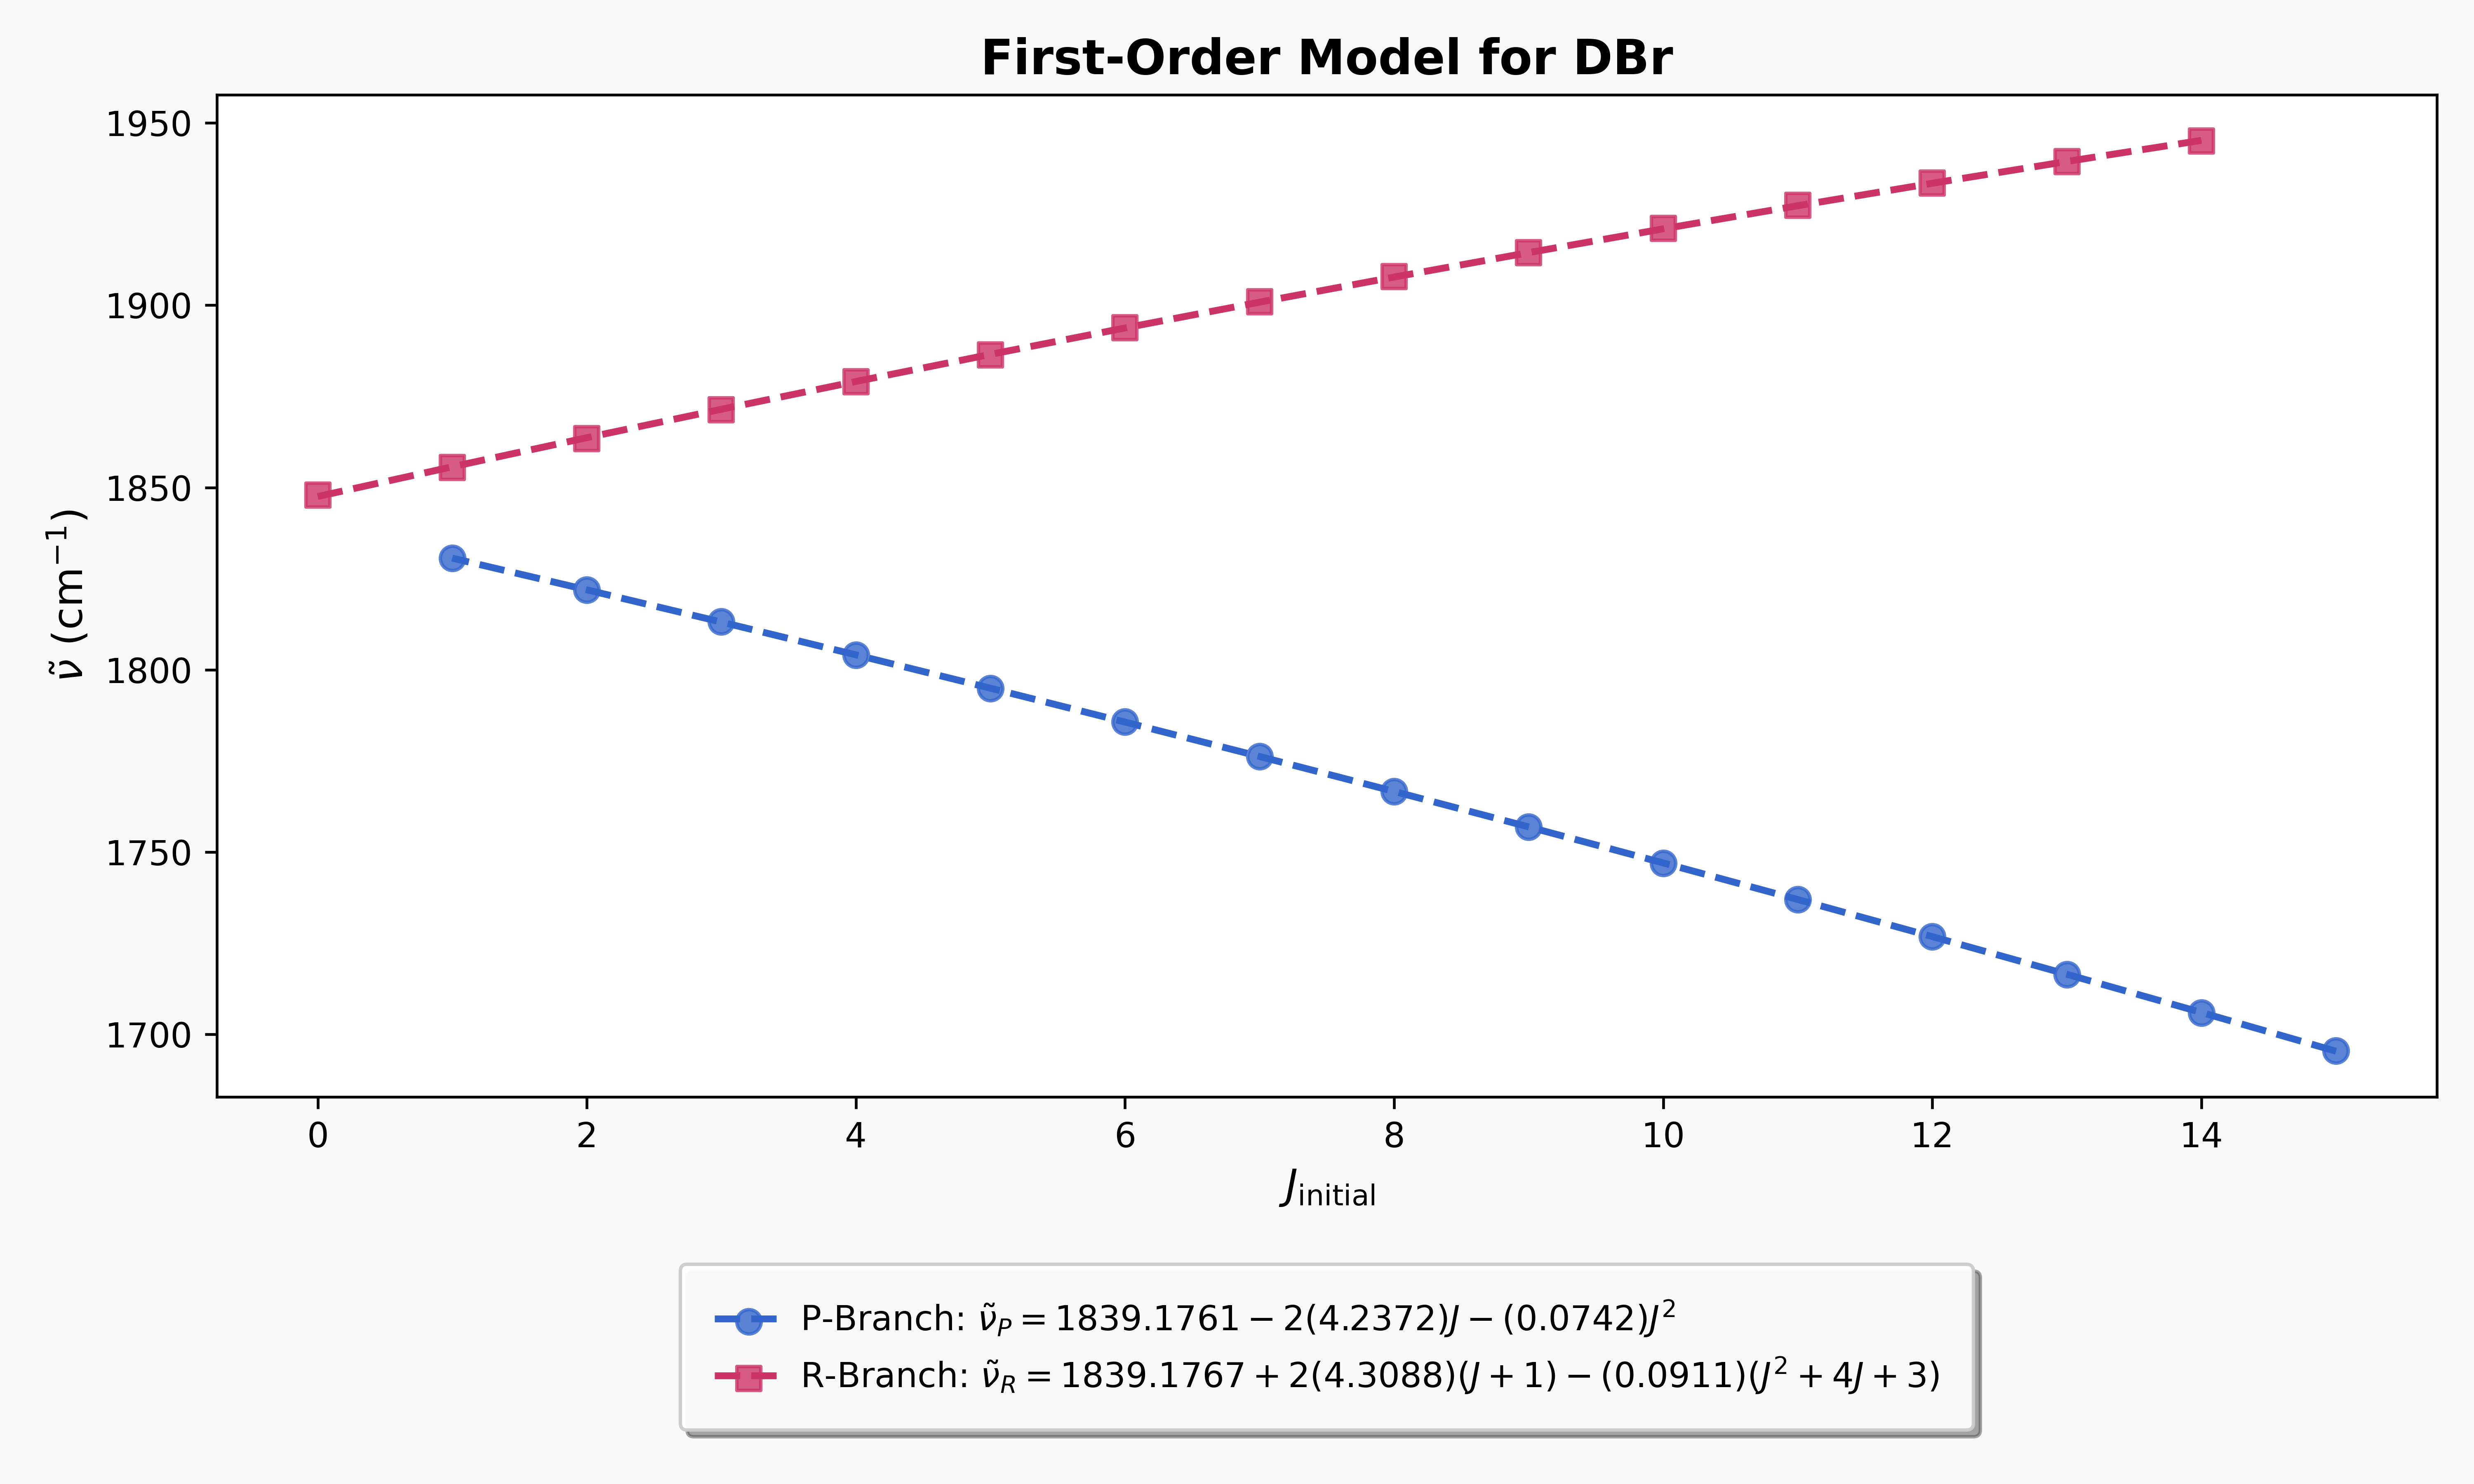
\includegraphics[width=\linewidth]{example-analysis/dbr-first-order-fit.png}
        \caption*{\mbox{}}
    \end{minipage}
    \begin{minipage}[t]{\textwidth}
            \centering
            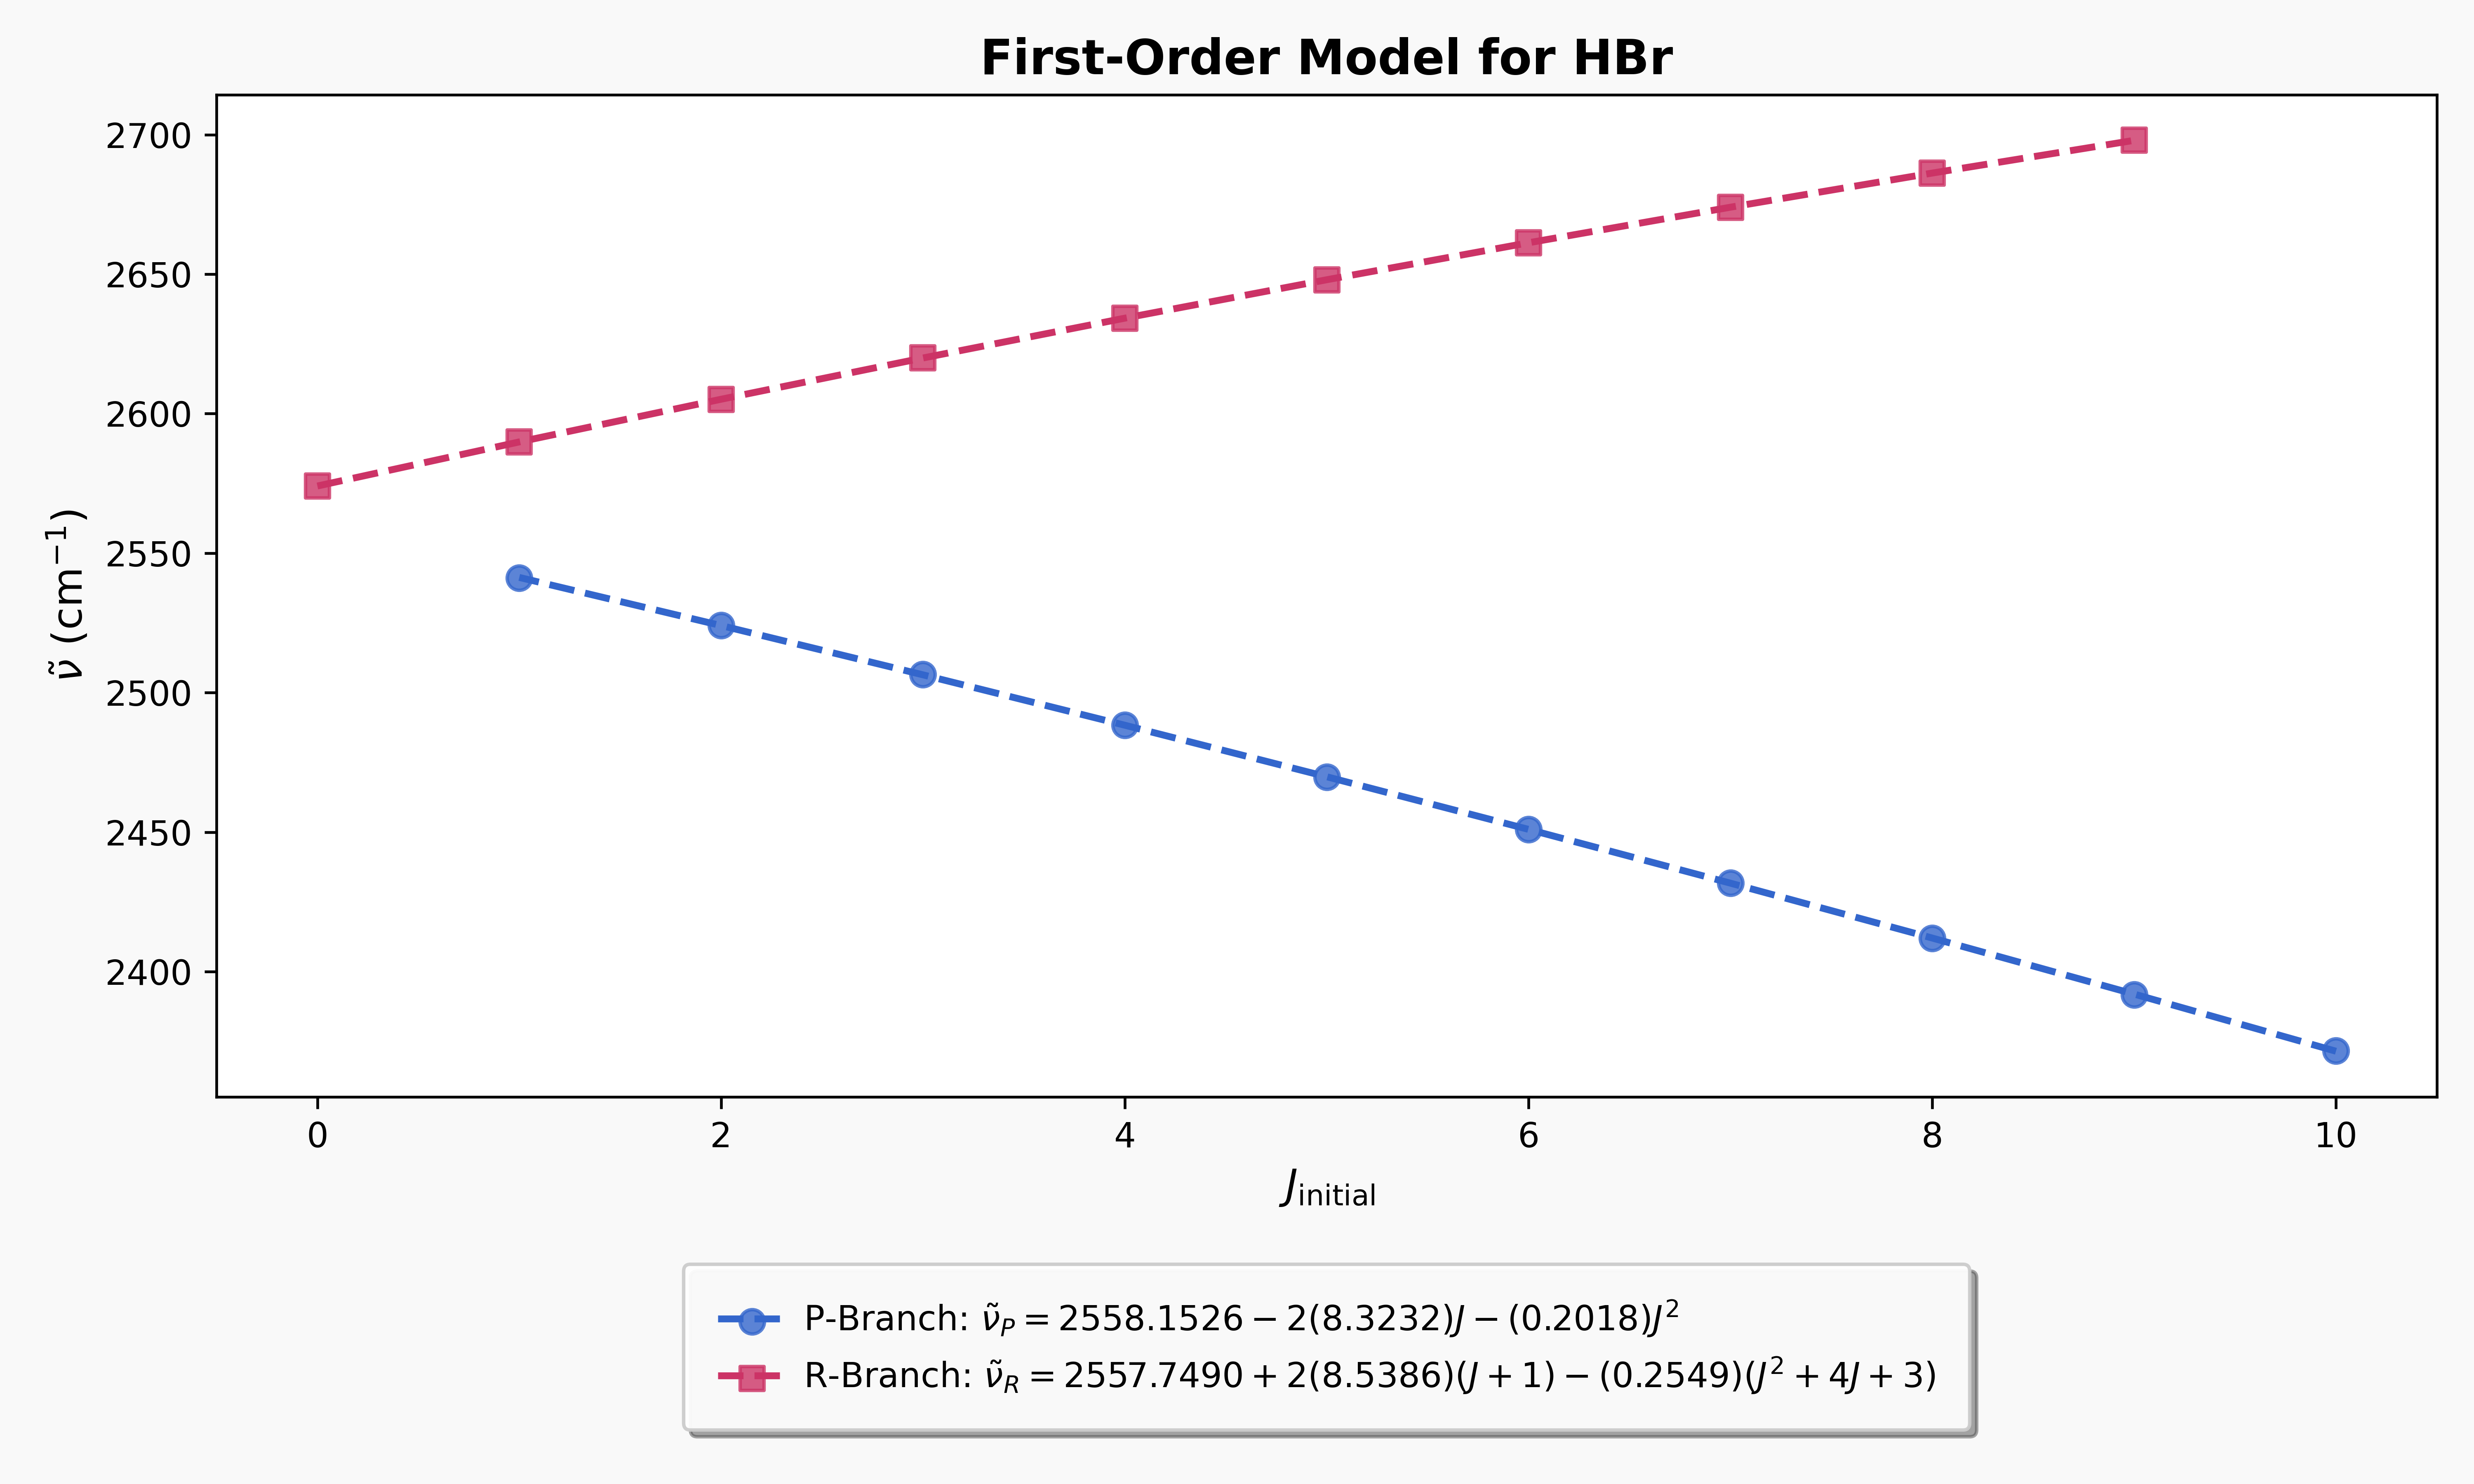
\includegraphics[width=\linewidth]{example-analysis/hbr-first-order-fit.png}
        \end{minipage}
    \end{figure}
\begin{figure}[htbp]
    \begin{minipage}[t]{\textwidth}
        \centering
        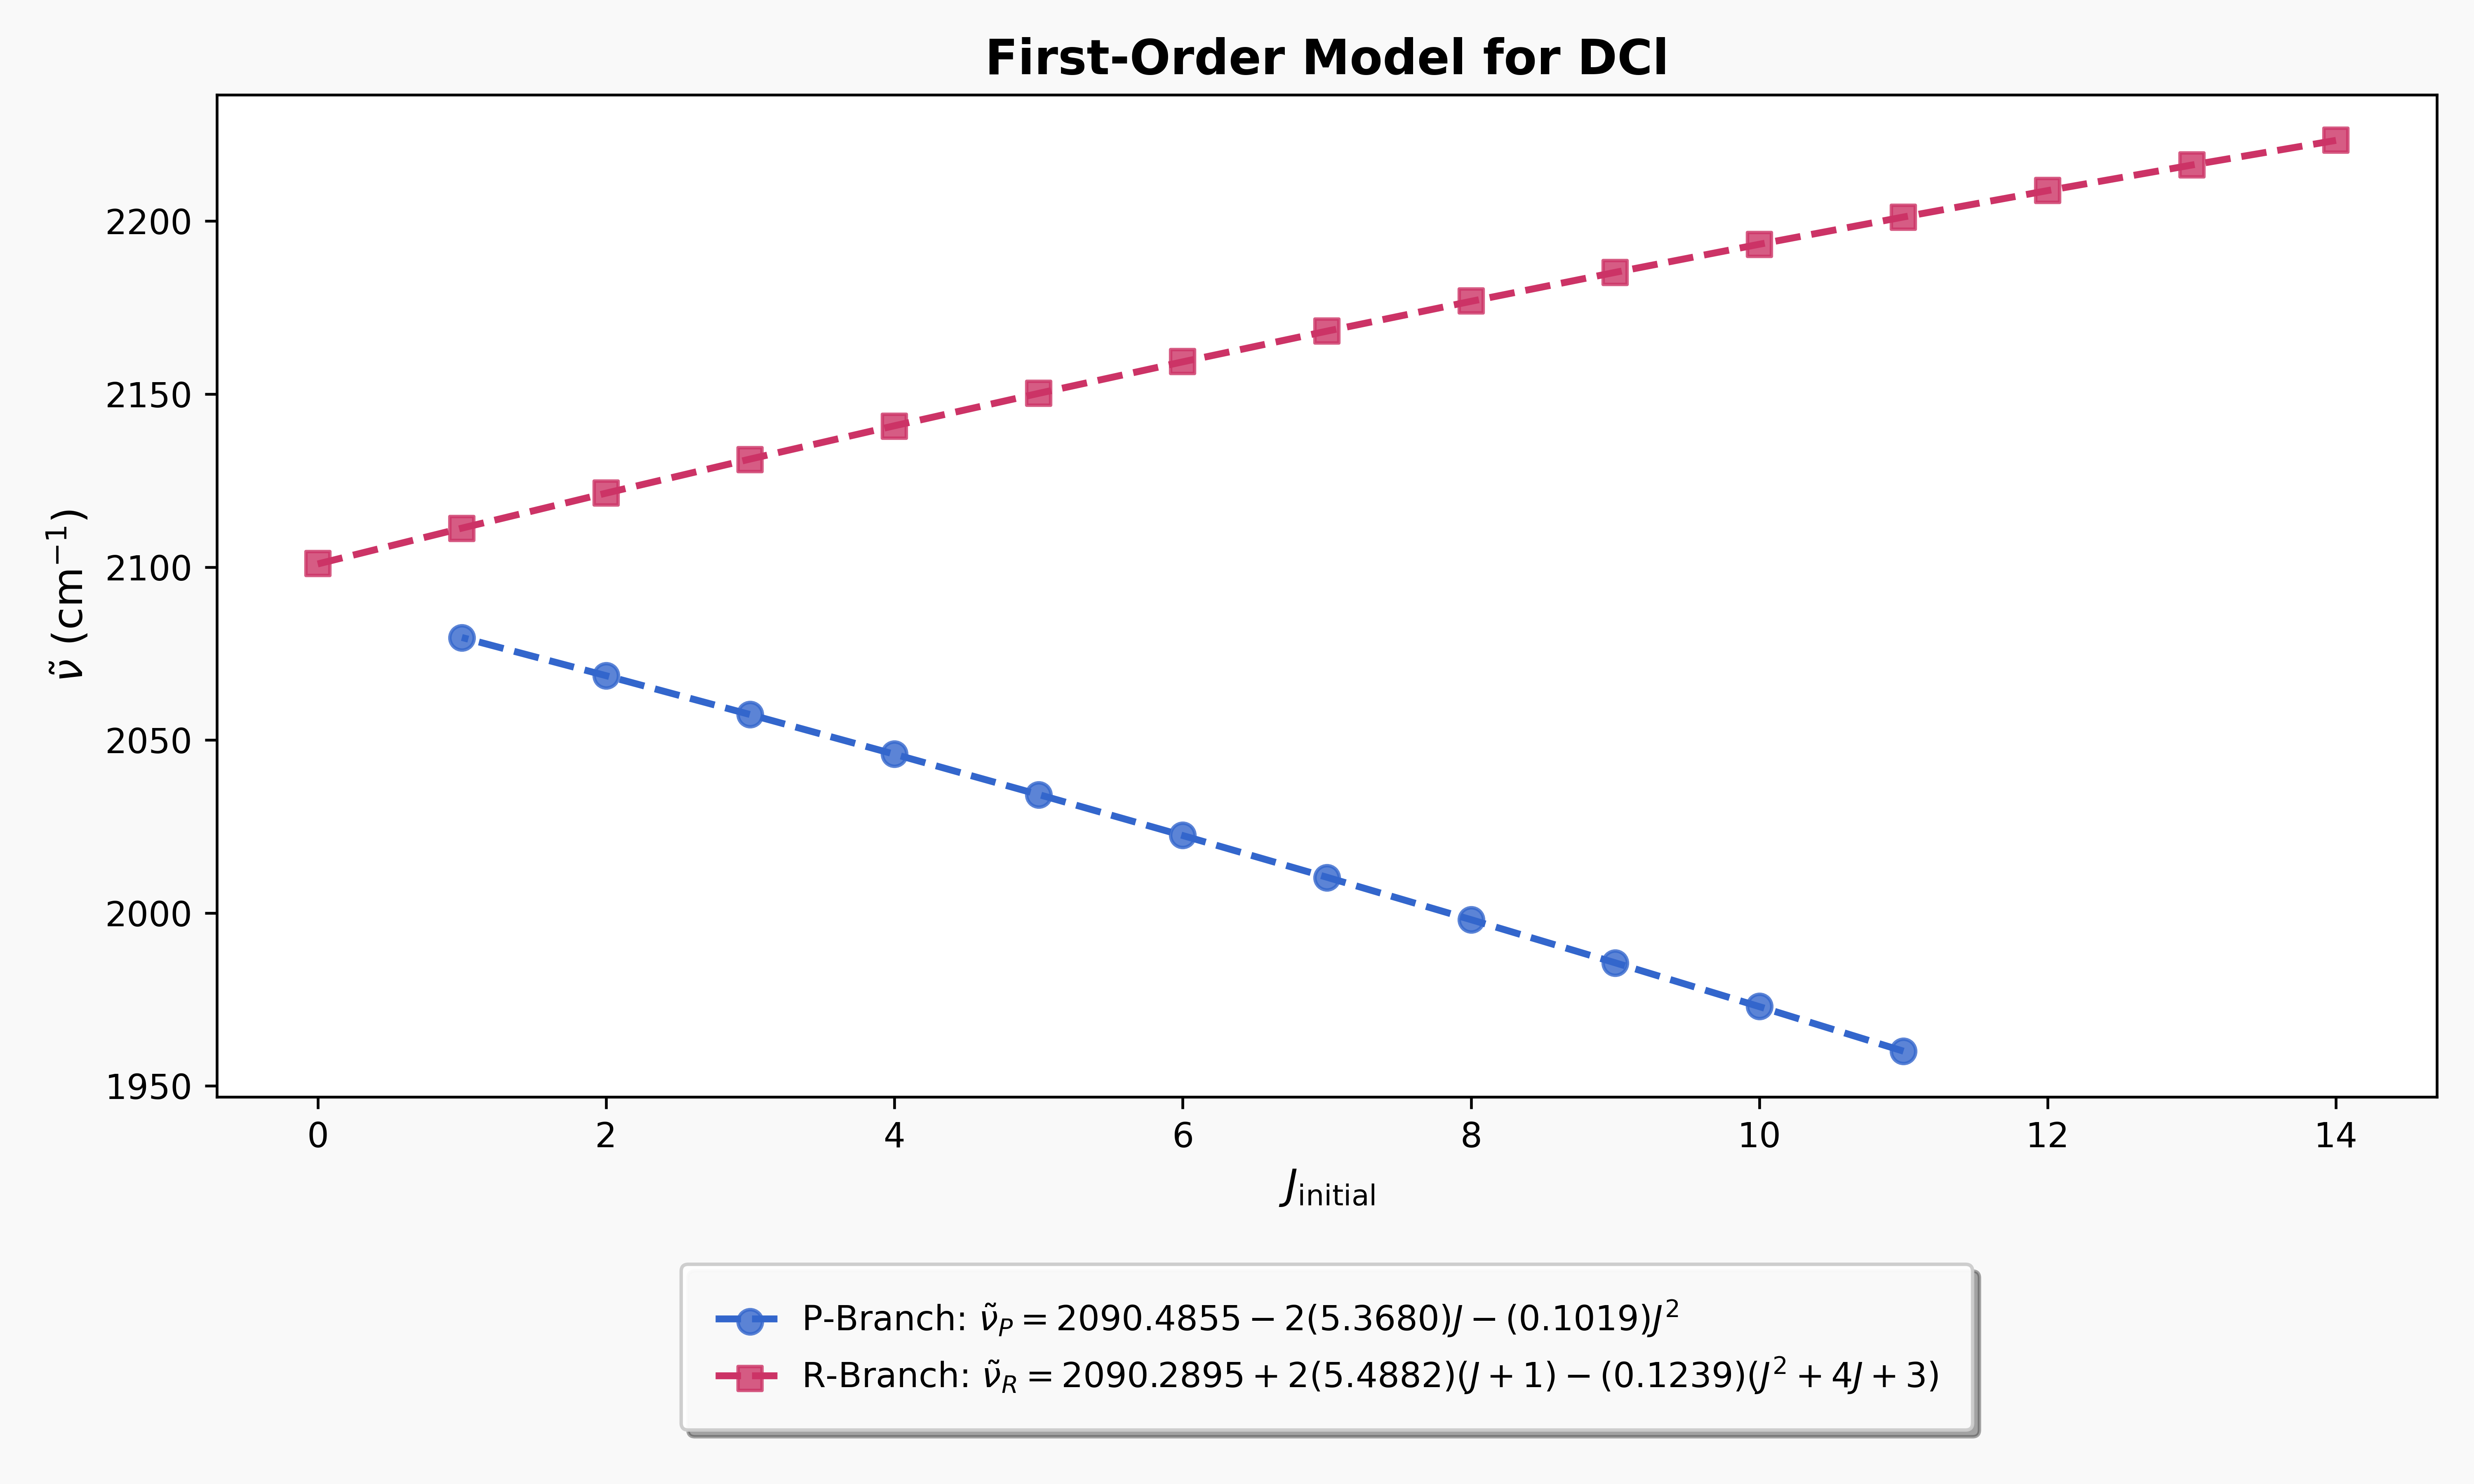
\includegraphics[width=\linewidth]{example-analysis/dcl-first-order-fit.png}
    \end{minipage}
\caption*{\mbox{}}
\begin{minipage}[t]{\textwidth}
        \centering
        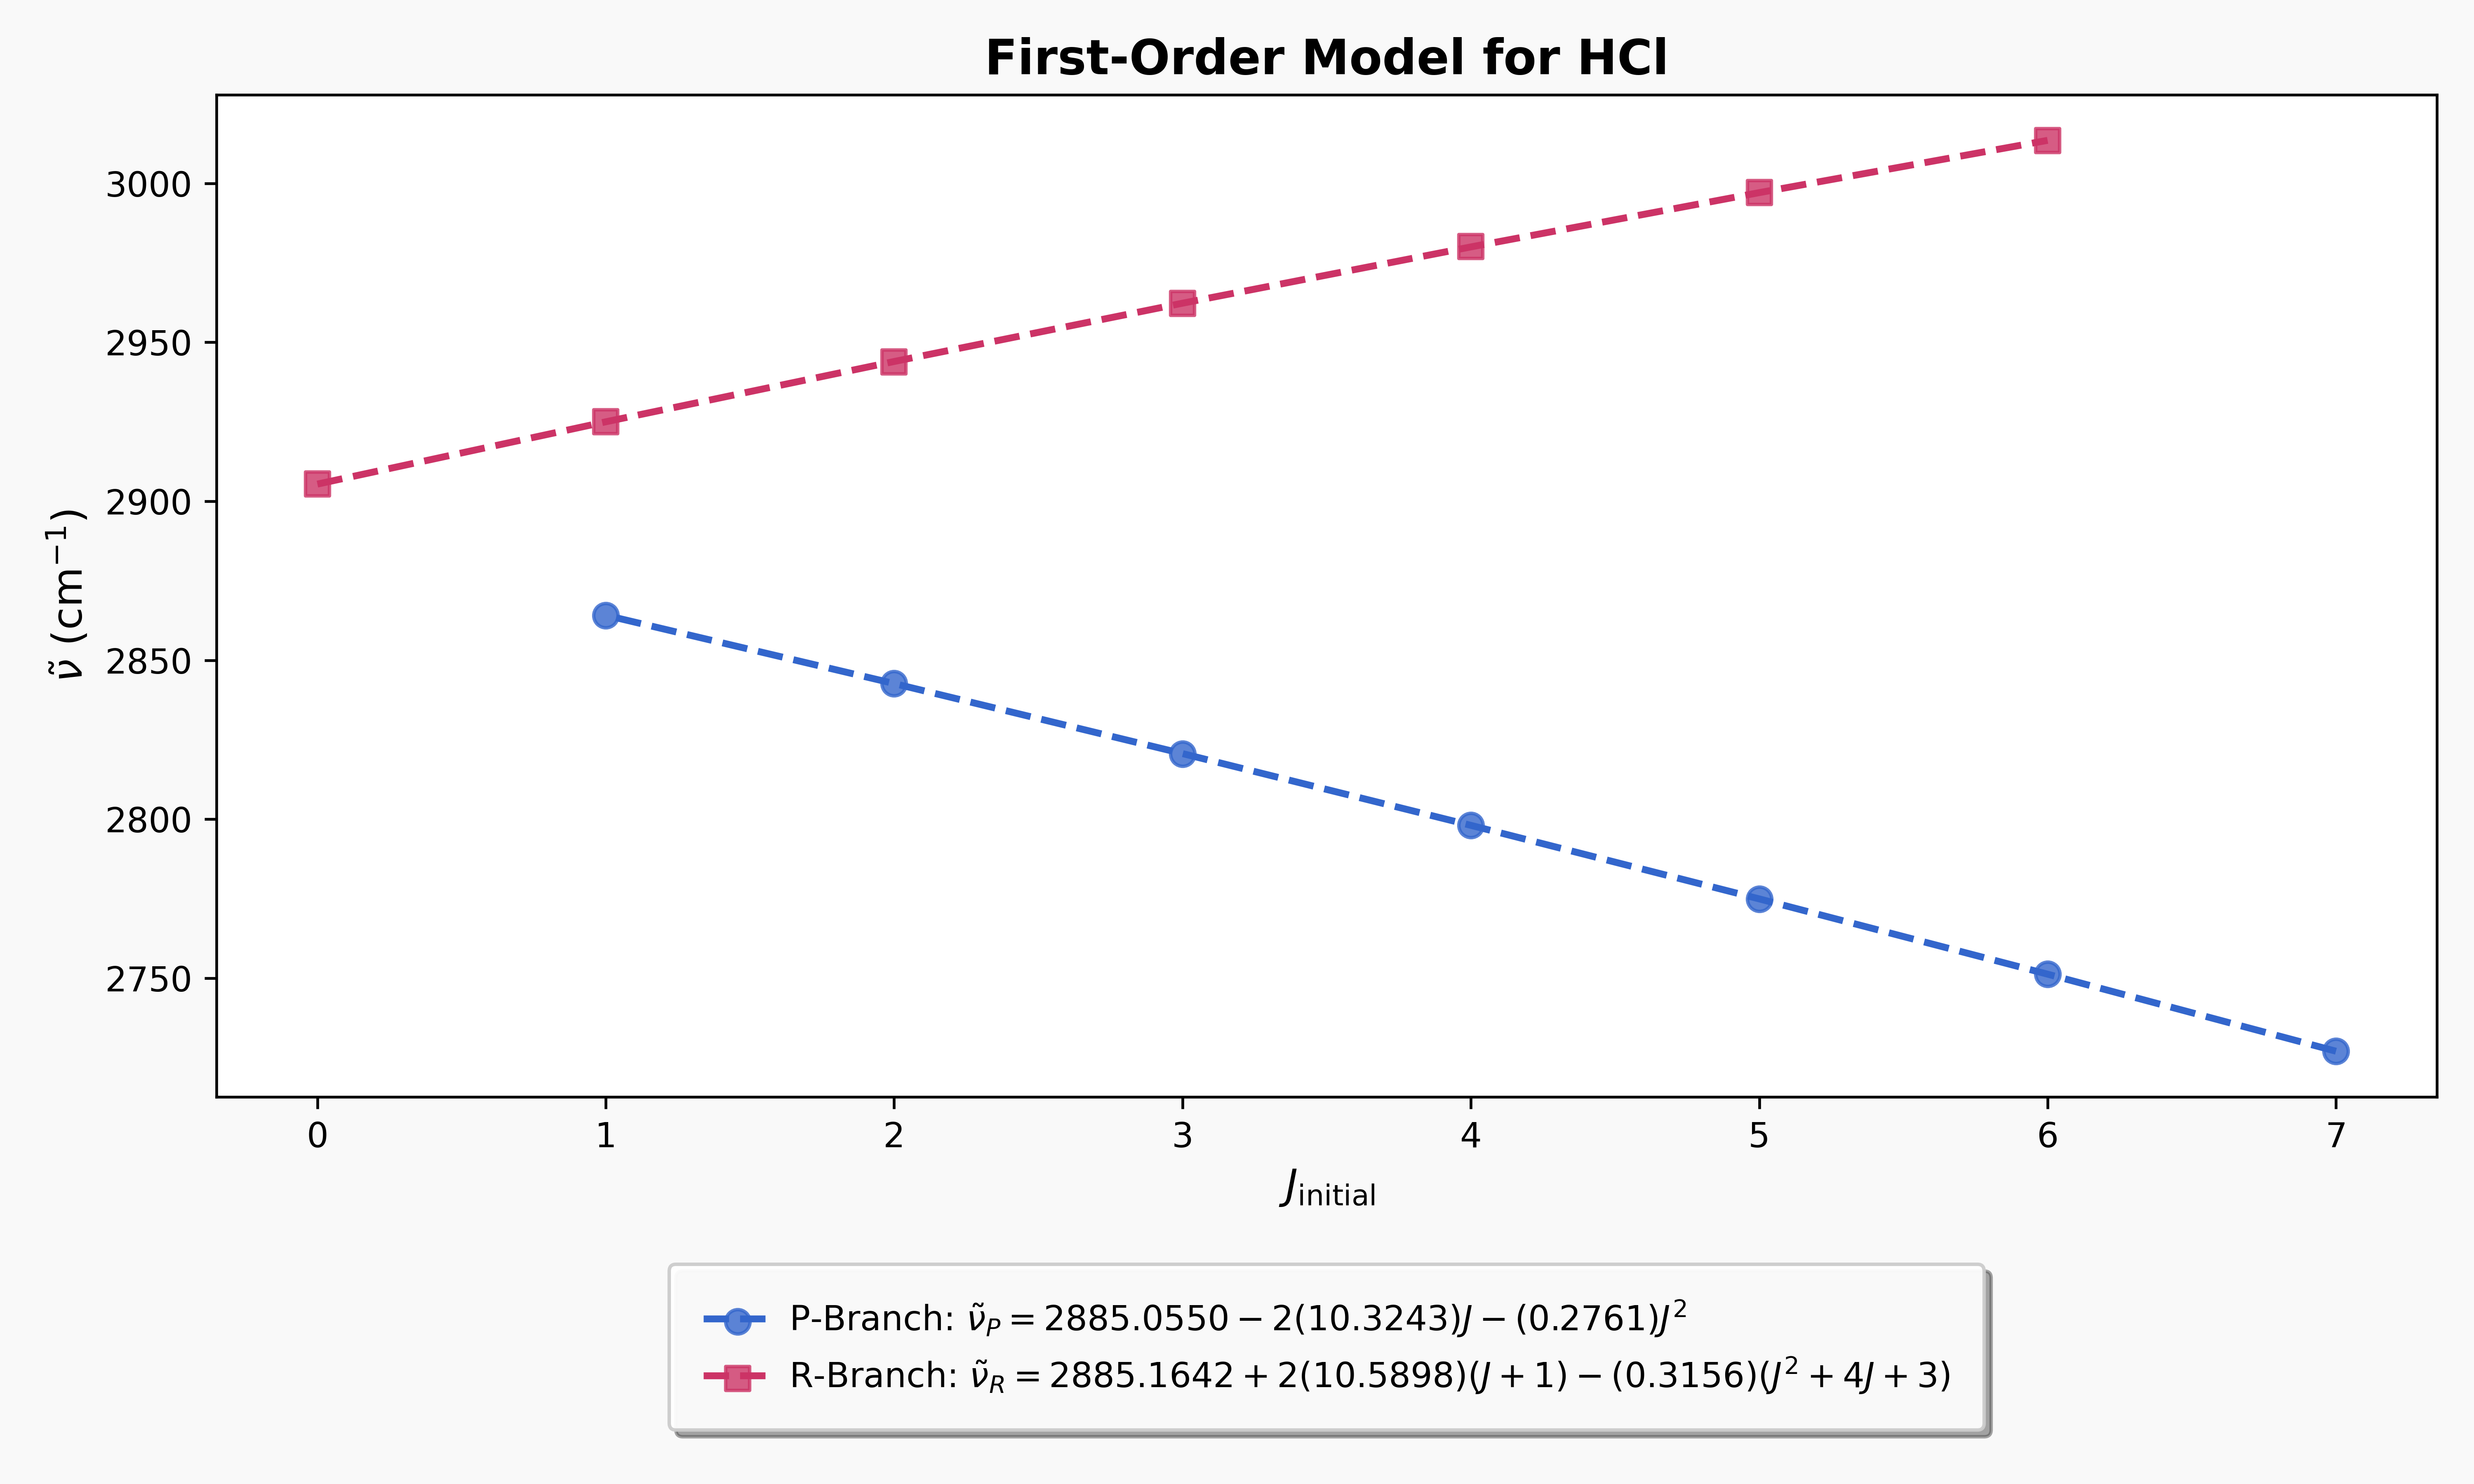
\includegraphics[width=\linewidth]{example-analysis/hcl-first-order-fit.png}
    \end{minipage}
\end{figure}
\begin{figure}[hbtp]
    ~\usesubsection{Background}
    The equation for the first order model is 
    \begin{align*}
        E_{1} &= h f_{0} \left(
            n + \frac{1}{2}
        \right) + hc BJ \left(
            J + 1
        \right) - h c \alpha \left(
            n + \frac{1}{2}
        \right)J\left(J+1\right)
    \end{align*}
    
    Like the zero order model, the first order approximation assumes the diatomic molecule consists of two systems: a simple harmonic oscillator (SHO) representing the vibrational energy, and a rigid rotator (RR) representing the rotational energy.  In reality the two systems are not isolated systems, since the bond length and angular frequency are coupled
    to both vibration and rotation. The first order model 
    therefore introduces a second term, \(\alpha\), which 
    accounts for this. 
    Since the rotational constant, \(B\), is inversely proportional to the bond length, \(\alpha\) will adjust the value of the rotational constant by accounting for larger non-ideal bond lengths. The magnitude of \(\alpha\) is affected by the vibrational quantum number, \(n\), since at higher vibrational energies the bond length will increase, and similarly the vibrational quantum number, \(J\). 
    The rotational energy of the molecule contributes a small proportion of the 
    total energy w.r.t. the contribution from vibrational energy. Therefore, 
    \(\alpha\) will be small when compared to B.
    The peak in a rovib spectra is thus the difference between sum of the change in vibrational energy and the change in rotational energy, and the coupling factor. 

    ~\usesubsection{P-Branch Derivations}
    The first order energies for the P-Branch are given by
\begin{align*}
    \Delta E_{\alpha, P} &= E\left(
        n + 1, J - 1
    \right)_{\alpha}
    - E\left(n,J\right)_{\alpha} \\
    &= h c \alpha \left(
        n + 1 + \frac{1}{2}
    \right)\left(J-1\right)\left(J-1+1\right)
    - h c \alpha \left(
        n + \frac{1}{2}
    \right)\left(J\left(J + 1\right)\right) \\
    &= h c \alpha \left[
        \left(
            n + \frac{3}{2}
        \right) \left(
            J^2 - J        
        \right)
        - \left(
            n + \frac{1}{2}
        \right) \left(
            J^2 + J
        \right)
    \right] \\
    &= h c \alpha \left[
        J^2n + \frac{3J^2}{2} - Jn 
        - \frac{3J}{2} - J^2 n - Jn 
        - \frac{J^2}{2} \frac{J}{2}
    \right] \\
    &= hc \alpha J \left(
        J - 2\left(n + 1\right)
    \right) \\
    \end{align*}
    With the position of the peaks given by
    \begin{align*}
    \Delta E_{1, P} &= \Delta E_{n} + \Delta E_{J, P} - \Delta E_{\alpha, P} \\
        \Delta E_{1, P} &= hf_{0} -hc\left(2BJ\right) - hc \alpha J \left(
            J - 2\left(n + 1\right)
        \right) \\
        \frac{\Delta E_{1, P}}{hc} &= \frac{f_0}{c} 
        - J\left[
            2B + \alpha\left(
                J - 2\left(n + 1\right)
            \right)
        \right] \\
        \tilde{\nu}_P &= \tilde{\nu}_0 - J\left[
            2B + \alpha\left(
                J - 2\left(n + 1\right)
            \right)
        \right] \\
        \text{\emph{Sub} \(n = 0\):}\quad
        \tilde{\nu}_{P} &= \tilde{\nu}_{0} - 2BJ - 
        \alpha J^2 \quad  \\
\end{align*}
\end{figure}
\begin{figure}[hbtp]
    ~\usesubsection{R-Branch Derivations}
    The first order energies for the R-branch are given by
\begin{align*}
        \Delta E_{\alpha, R} &= E\left(
            n + 1, J + 1
        \right)_{\alpha}
        - E\left(n,J\right)_{\alpha} \\
        &= h c \alpha \left(
            n + 1 + \frac{1}{2}
        \right)\left(J+1\right)\left(J+1+1\right)
        - h c \alpha \left(
            n + \frac{1}{2}
        \right)\left(J\left(J + 1\right)\right) \\
        &= h c \alpha \left[
            \left(
                n + \frac{3}{2}
            \right)\left(J^2 + 3J + 2\right)
            - \left(n + \frac{1}{2}\right)
            \left(J^2 + J\right)
        \right] \\
        &= h c \alpha \left[
            J^2 + 4J + 2Jn +2n + 3   
        \right] \\
        &= h c \alpha \left[
            J \left(
                J + 4
            \right) + 2n \left(
                J + 1
            \right) + 3
        \right] \\
    \end{align*}
    With the position of the peaks given by
    \begin{align*}
        \Delta E_{1, R} &= \Delta E_{n} + 
        \Delta E_{J, R} - \Delta E_{\alpha, R} \\
        \Delta E_{1, R} &= hf_{0} 
        + h c\left(2B \right)\left(J + 1\right)
        - h c \alpha \left[
            J \left(
                J + 4
            \right) + 2n \left(
                J + 1
            \right) + 3
        \right] \\
        \frac{\Delta E_{1, R}}{hc} &= \frac{f_0}{c}
        + 2B\left(J+1\right)
        - \alpha\left[
            J\left(J+4\right) + 2n\left(J+1\right) + 3
        \right] \\
        \tilde{\nu}_{R} &= \tilde{\nu}_0 + 2B\left(J+1\right)
        - \alpha\left[
            J\left(J+4\right) + 2n\left(J+1\right) + 3
        \right] \\
        \text{\emph{Sub} \(n = 0\):} \quad 
        \tilde{\nu}_{R} &= \tilde{\nu}_{0}
        + 2B\left(J + 1\right)
        - \alpha\left(J^2 + 4J + 3\right) \quad  \\
\end{align*}
~\usesubsection{Fundamental Wavenumber}
The first order fit describes the peak positions
of the R-Branch with   \(
\tilde{\nu} =  \tilde{\nu}_{0}
+ 2B\left(J + 1\right)
- \alpha\left(J^2 + 4J + 3\right) 
\) and for the P-branch we get \(
    \tilde{\nu} = \tilde{\nu}_{0} - 2BJ
\). After we perform a linear regression on the data for DBr, 
we get \(
\tilde{\nu}_{R} = 1839.1767 + 2\left(
    4.3088
\right)\left(
    J+1
\right) - \left(
    0.0911
\right) \left(
    J^2 + 4J + 3
\right)
\), and \(
\tilde{\nu}_{P} = 1839.1761 - 2\left(
    4.2372
\right)J - \left(
    0.0742
\right)^2
\). Calculating the average gives
\begin{align*}
    \tilde{\nu}_{0} &= \frac{\tilde{\nu}_{R} + \tilde{\nu}_P}{2} 
    = \frac{1839.1767 + 1839.1761}{2} 
    \approx 1839.1764 \mathrm{cm}^{-1} \\
    SD &= \sqrt{
        \frac{
            \left(
                1839.1767 - 1839.1764
            \right)^2
        + \left(
            1839.1761 - 1839.1764
        \right)^2
        }{2}
    } 
    \approx 0.0003 \mathrm{cm}^{-1} \\
    SE &= \frac{SD}{\sqrt{2}} 
    = \frac{0.0003}{\sqrt{2}} 
    \approx 0.0002 \mathrm{cm}^{-1} \\
    \mathbf{\tilde{\nu}}_{0} &= \mathbf{
        \left(
            1842.9 \pm 0.0002
        \right) cm^{-1}
    } \\
\end{align*}
\end{figure}
\begin{figure}[htbp]
    ~\usesubsection{Rotational Constant}
    \begin{align*}
        B &= \frac{B_{R} + B_{P}}{2} \\
        &= \frac{4.3088 + 4.2372}{2} \\
        &\approx 4.2730 \mathrm{cm}^{-1} \\
        SD &= \sqrt{
            \frac{
                \left(
                    4.3088 - 4.2730
                \right)^2
            + \left(
                4.2372 - 4.2730
            \right)^2
            }{2}
        } \\
        &\approx 0.0358 \mathrm{cm}^{-1} \\
        SE &= \frac{SD}{\sqrt{2}} \\
        &= \frac{0.0358}{\sqrt{2}} \\ 
        & \approx 0.0253 \mathrm{cm}^{-1} \\
        \mathbf{B} &= \mathbf{
            \left(
                4.2730 \pm 0.0253
            \right) cm^{-1}
        } \\
    \end{align*}
    ~\usesubsection{Rotational-Vibrational Coupling Constant}
    \begin{align*}
        \alpha &= \frac{\alpha_{R} + \alpha_{P}}{2} \\
        &= \frac{0.0911 + 0.0742}{2} \\
        &= 0.0826 \mathrm{cm}^{-1} \\
        SD &= \sqrt{
            \frac{
                \left(
                    0.0911 - 0.0826
                \right)^2
            + \left(
                0.0742 - 0.0826
            \right)^2
            }{2}
        } \\
        &= 0.00845015 \mathrm{cm}^{-1} \\
        SE &= \frac{SD}{\sqrt{2}} \\
        &= \frac{0.00845015}{\sqrt{2}} \\ 
        & \approx 0.006 \mathrm{cm}^{-1} \\
        \mathbf{\alpha} &\mathbf{= 
            \left(
                0.0826 \pm 0.006
            \right) cm^{-1}
        } \\
    \end{align*}
\end{figure}
\begin{figure}[htbp]
~\usesubsection{Equilibrium Radius}    
\begin{align*}
    r_{e, R} &= \sqrt{
        \frac{h}{8 \pi^2 c \mu_{\text{\scriptsize DBr}}  B_{R}}} \\
    &= \sqrt{
    \frac{0.0399031221 \mathring{A}^2 \cdot \nicefrac{\mathrm{amu}}{\mathrm{fs}}}{
    \left(
        8 \pi^2
    \right)    
    \left(
        2.99792458\times 10^{3}\nicefrac{\mathring{A}}{\mathrm{fs}}
    \right) \left(
        1.9646 \cdot \mathrm{amu}
    \right)
    \left(
        4.3088 \times 10^{-8} \mathring{A}^{-1}
    \right) 
    }}\\
    &\approx 1.411 \mathring{A} \\
    r_{e, P} &= \sqrt{
        \frac{h}{8 \pi^2 c \mu_{\text{\scriptsize DBr}}  B_{P}}} \\
    &= \sqrt{
    \frac{0.0399031221 \mathring{A}^2 \cdot \nicefrac{\mathrm{amu}}{\mathrm{fs}}}{
    \left(
        8 \pi^2
    \right)    
    \left(
        2.99792458\times 10^{3}\nicefrac{\mathring{A}}{\mathrm{fs}}
    \right) \left(
        1.9646 \cdot \mathrm{amu}
    \right)
    \left(
        4.2372 \times 10^{-8} \mathring{A}^{-1}
    \right) 
    }}\\
    &\approx 1.423 \mathring{A} \\
    r_{e} &= \frac{ r_{e, R} + r_{e, P}}{2} \\
    &= \frac{1.411 + 1.423}{2} \\
    &\approx 1.417 \mathring{A} \\
    SD &= \sqrt{
        \frac{
            \left(
                1.411 - 1.417
            \right)^2
        + \left(
            1.423 - 1.417
        \right)^2
        }{2}
    } \\
    &\approx 0.006 \mathring{A} \\
    SE &= \frac{SD}{\sqrt{2}} \\
    &= \frac{0.006}{\sqrt{2}} \\
    & \approx 0.0042 \mathring{A} \\
    \mathbf{r_e} &= \mathbf{
        \left(
            1.417 \pm 0.0042
        \right) \mathring{A}
    } \\
\end{align*}
~\usesubsection{Moment of Inertia}
The moment of inertia for the P-branch is \(
I_{P} \approx 3.9785 \mathrm{amu} \cdot \mathring{A}^2
\) and for the R-Branch \(
I_{R} \approx 3.9124 \mathrm{amu} \cdot \mathring{A}^2
\). This gives an average of \(
\mathbf{\left(
    3.9454 \pm 0.0234
\right) amu \cdot \mathring{A}^2}
\)
\end{figure}

\newpage
\begin{figure}[hbtp]
    ~\usesection{Second Order Model}
    \centering
    \begin{minipage}[t]{\textwidth}
        \centering
        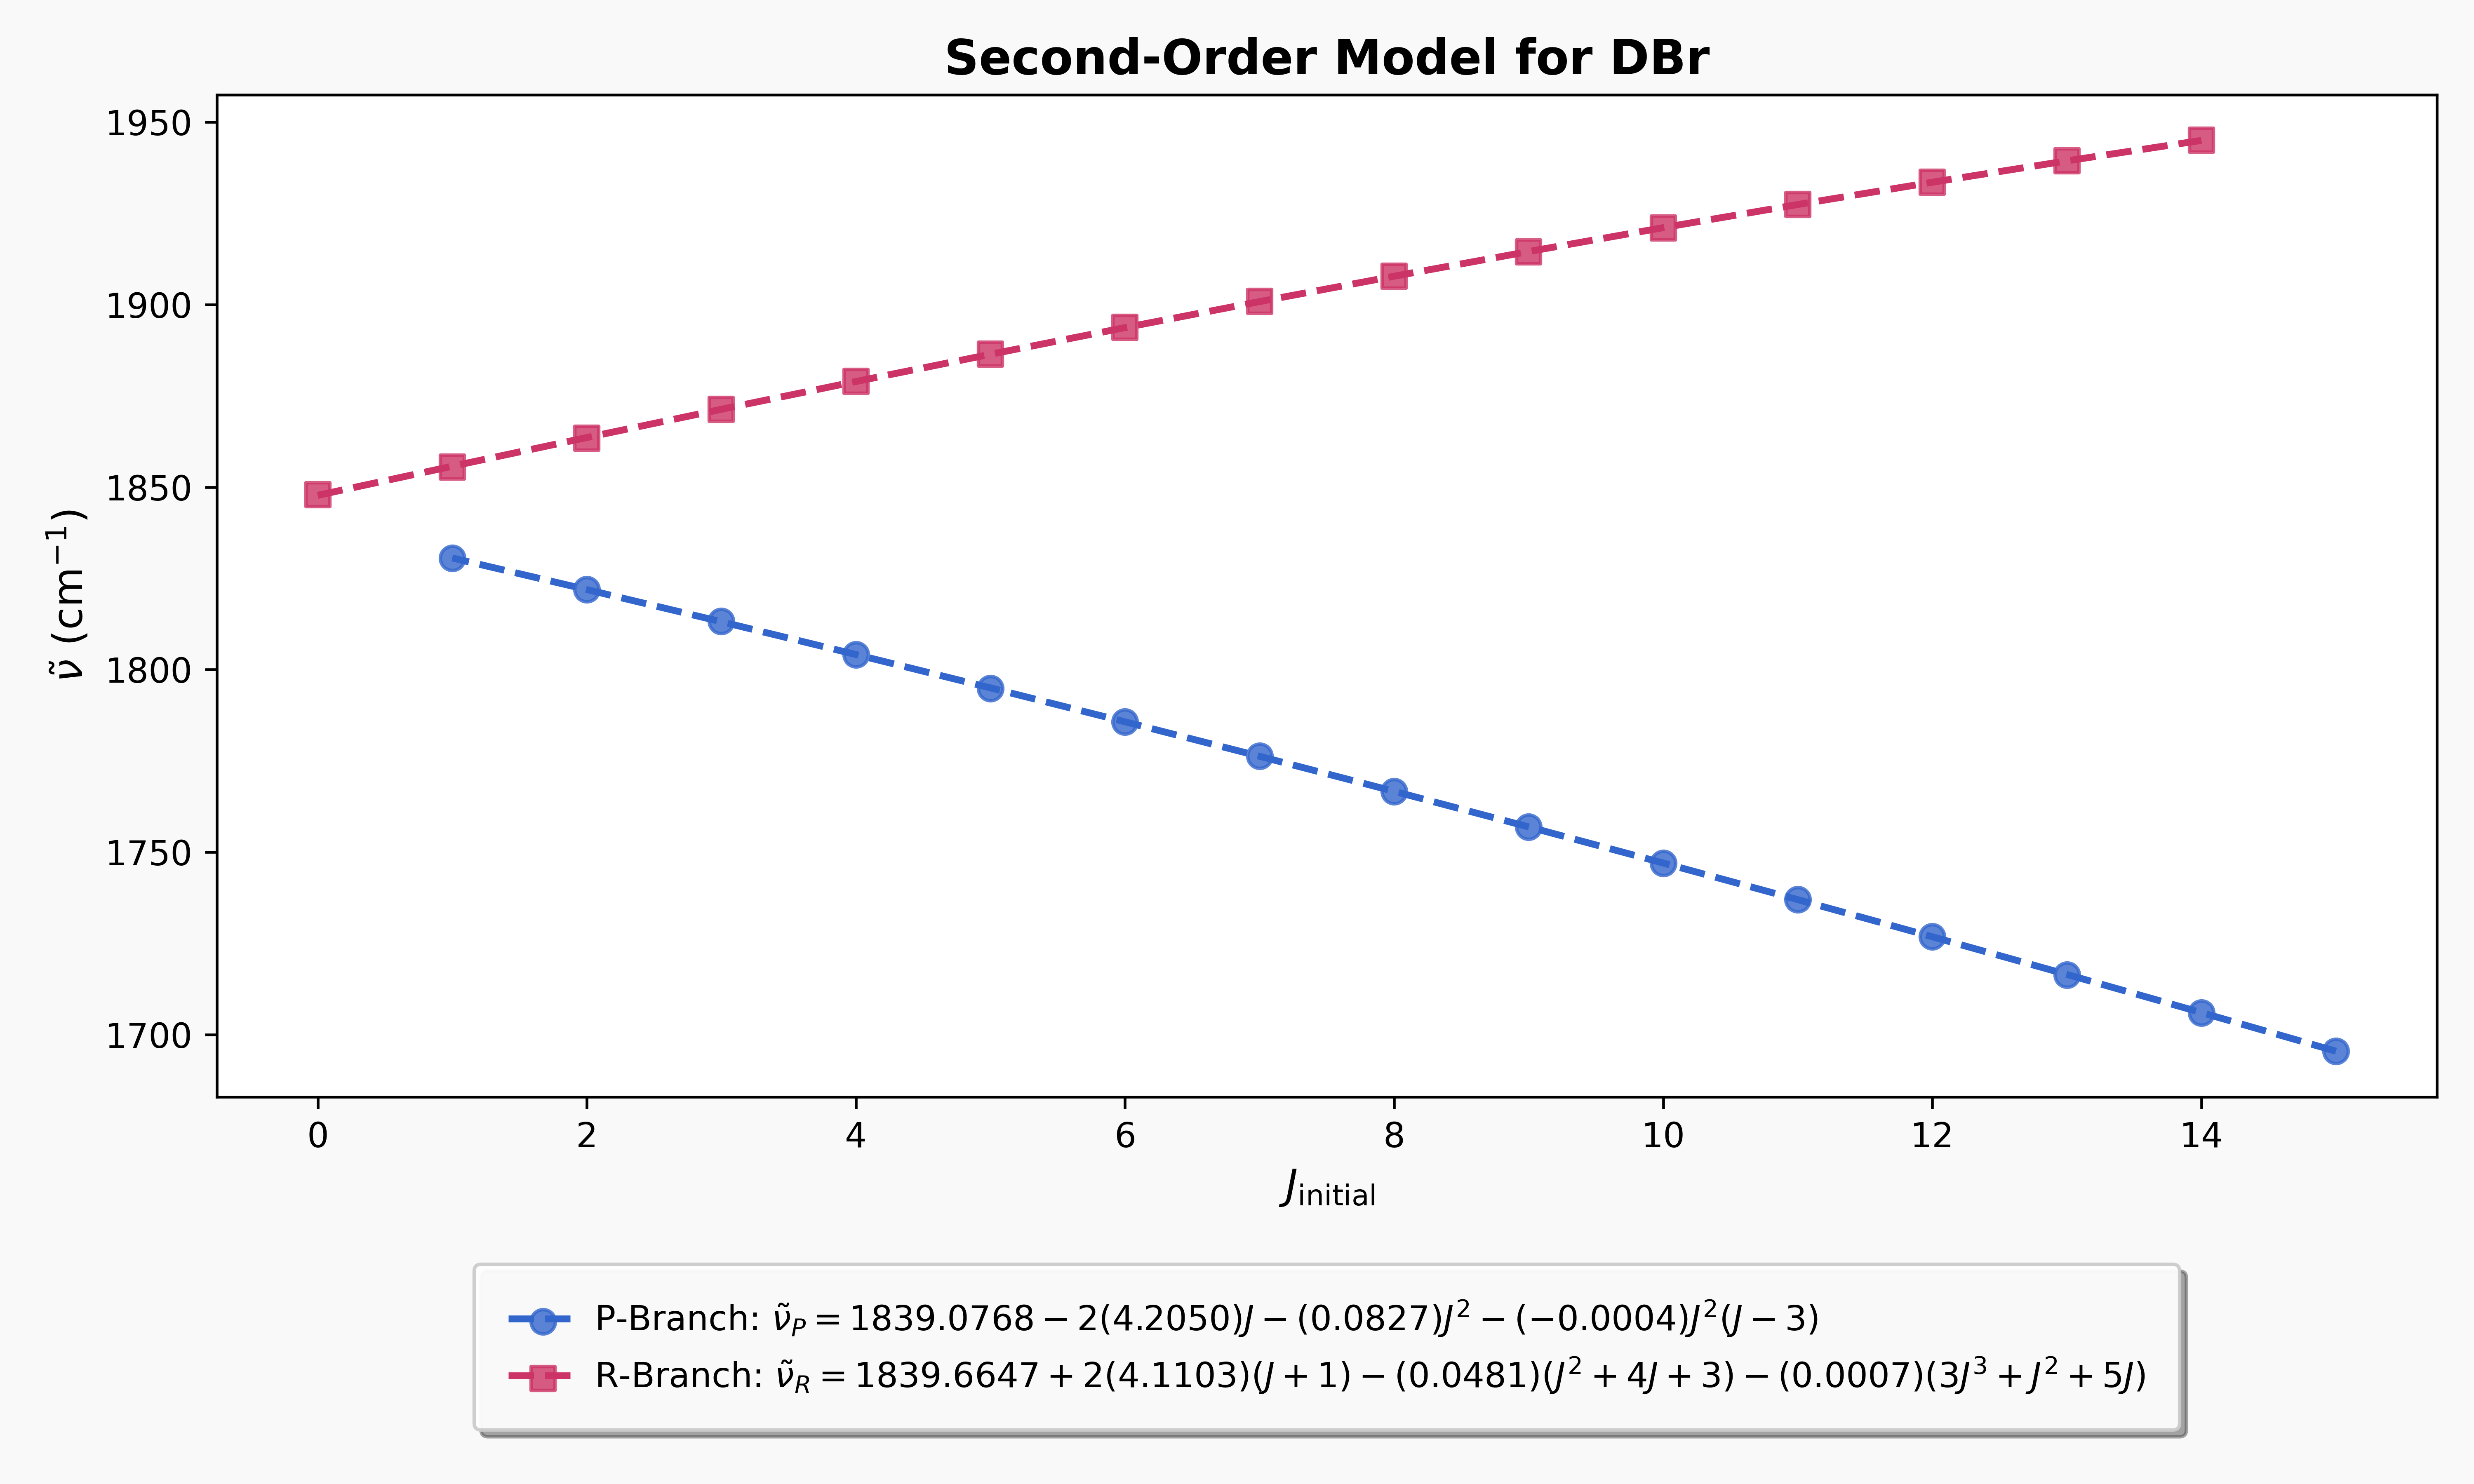
\includegraphics[width=\linewidth]{example-analysis/dbr-second-order-fit.png}
        \caption*{\mbox{}}
    \end{minipage}
    \begin{minipage}[t]{\textwidth}
            \centering
            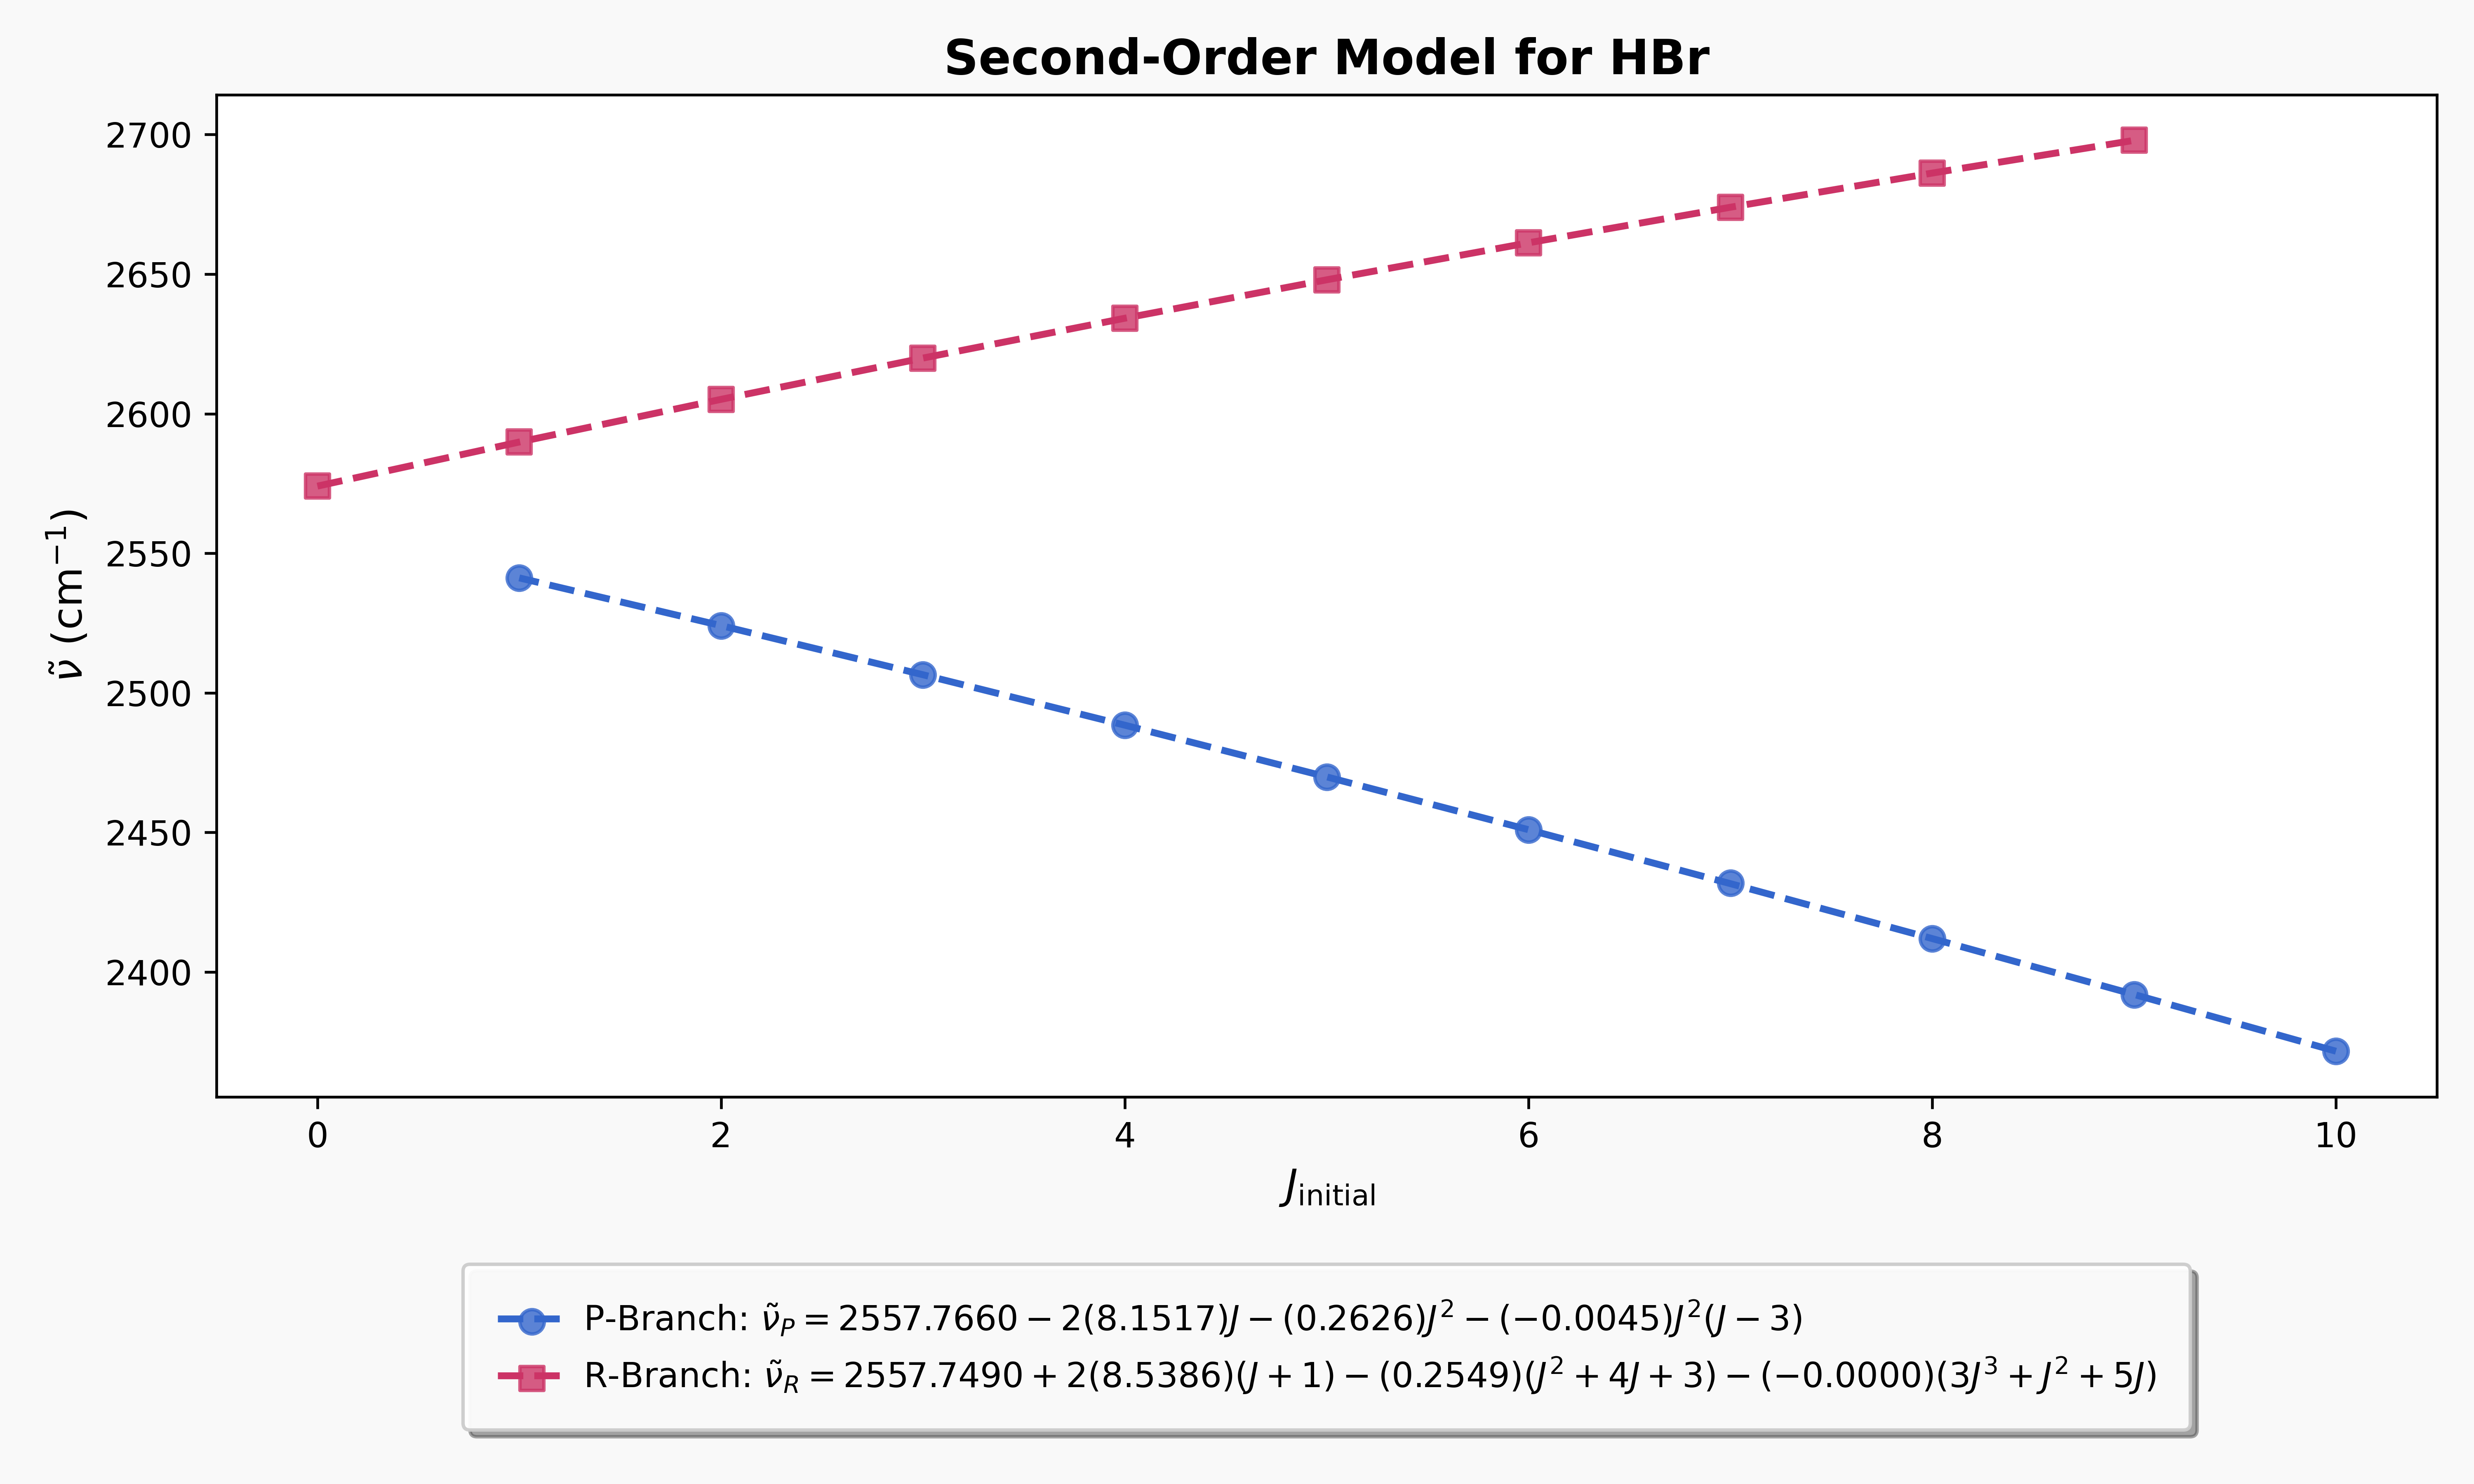
\includegraphics[width=\linewidth]{example-analysis/hbr-second-order-fit.png}
        \end{minipage}
    \end{figure}
\begin{figure}[htbp]
    \begin{minipage}[t]{\textwidth}
        \centering
        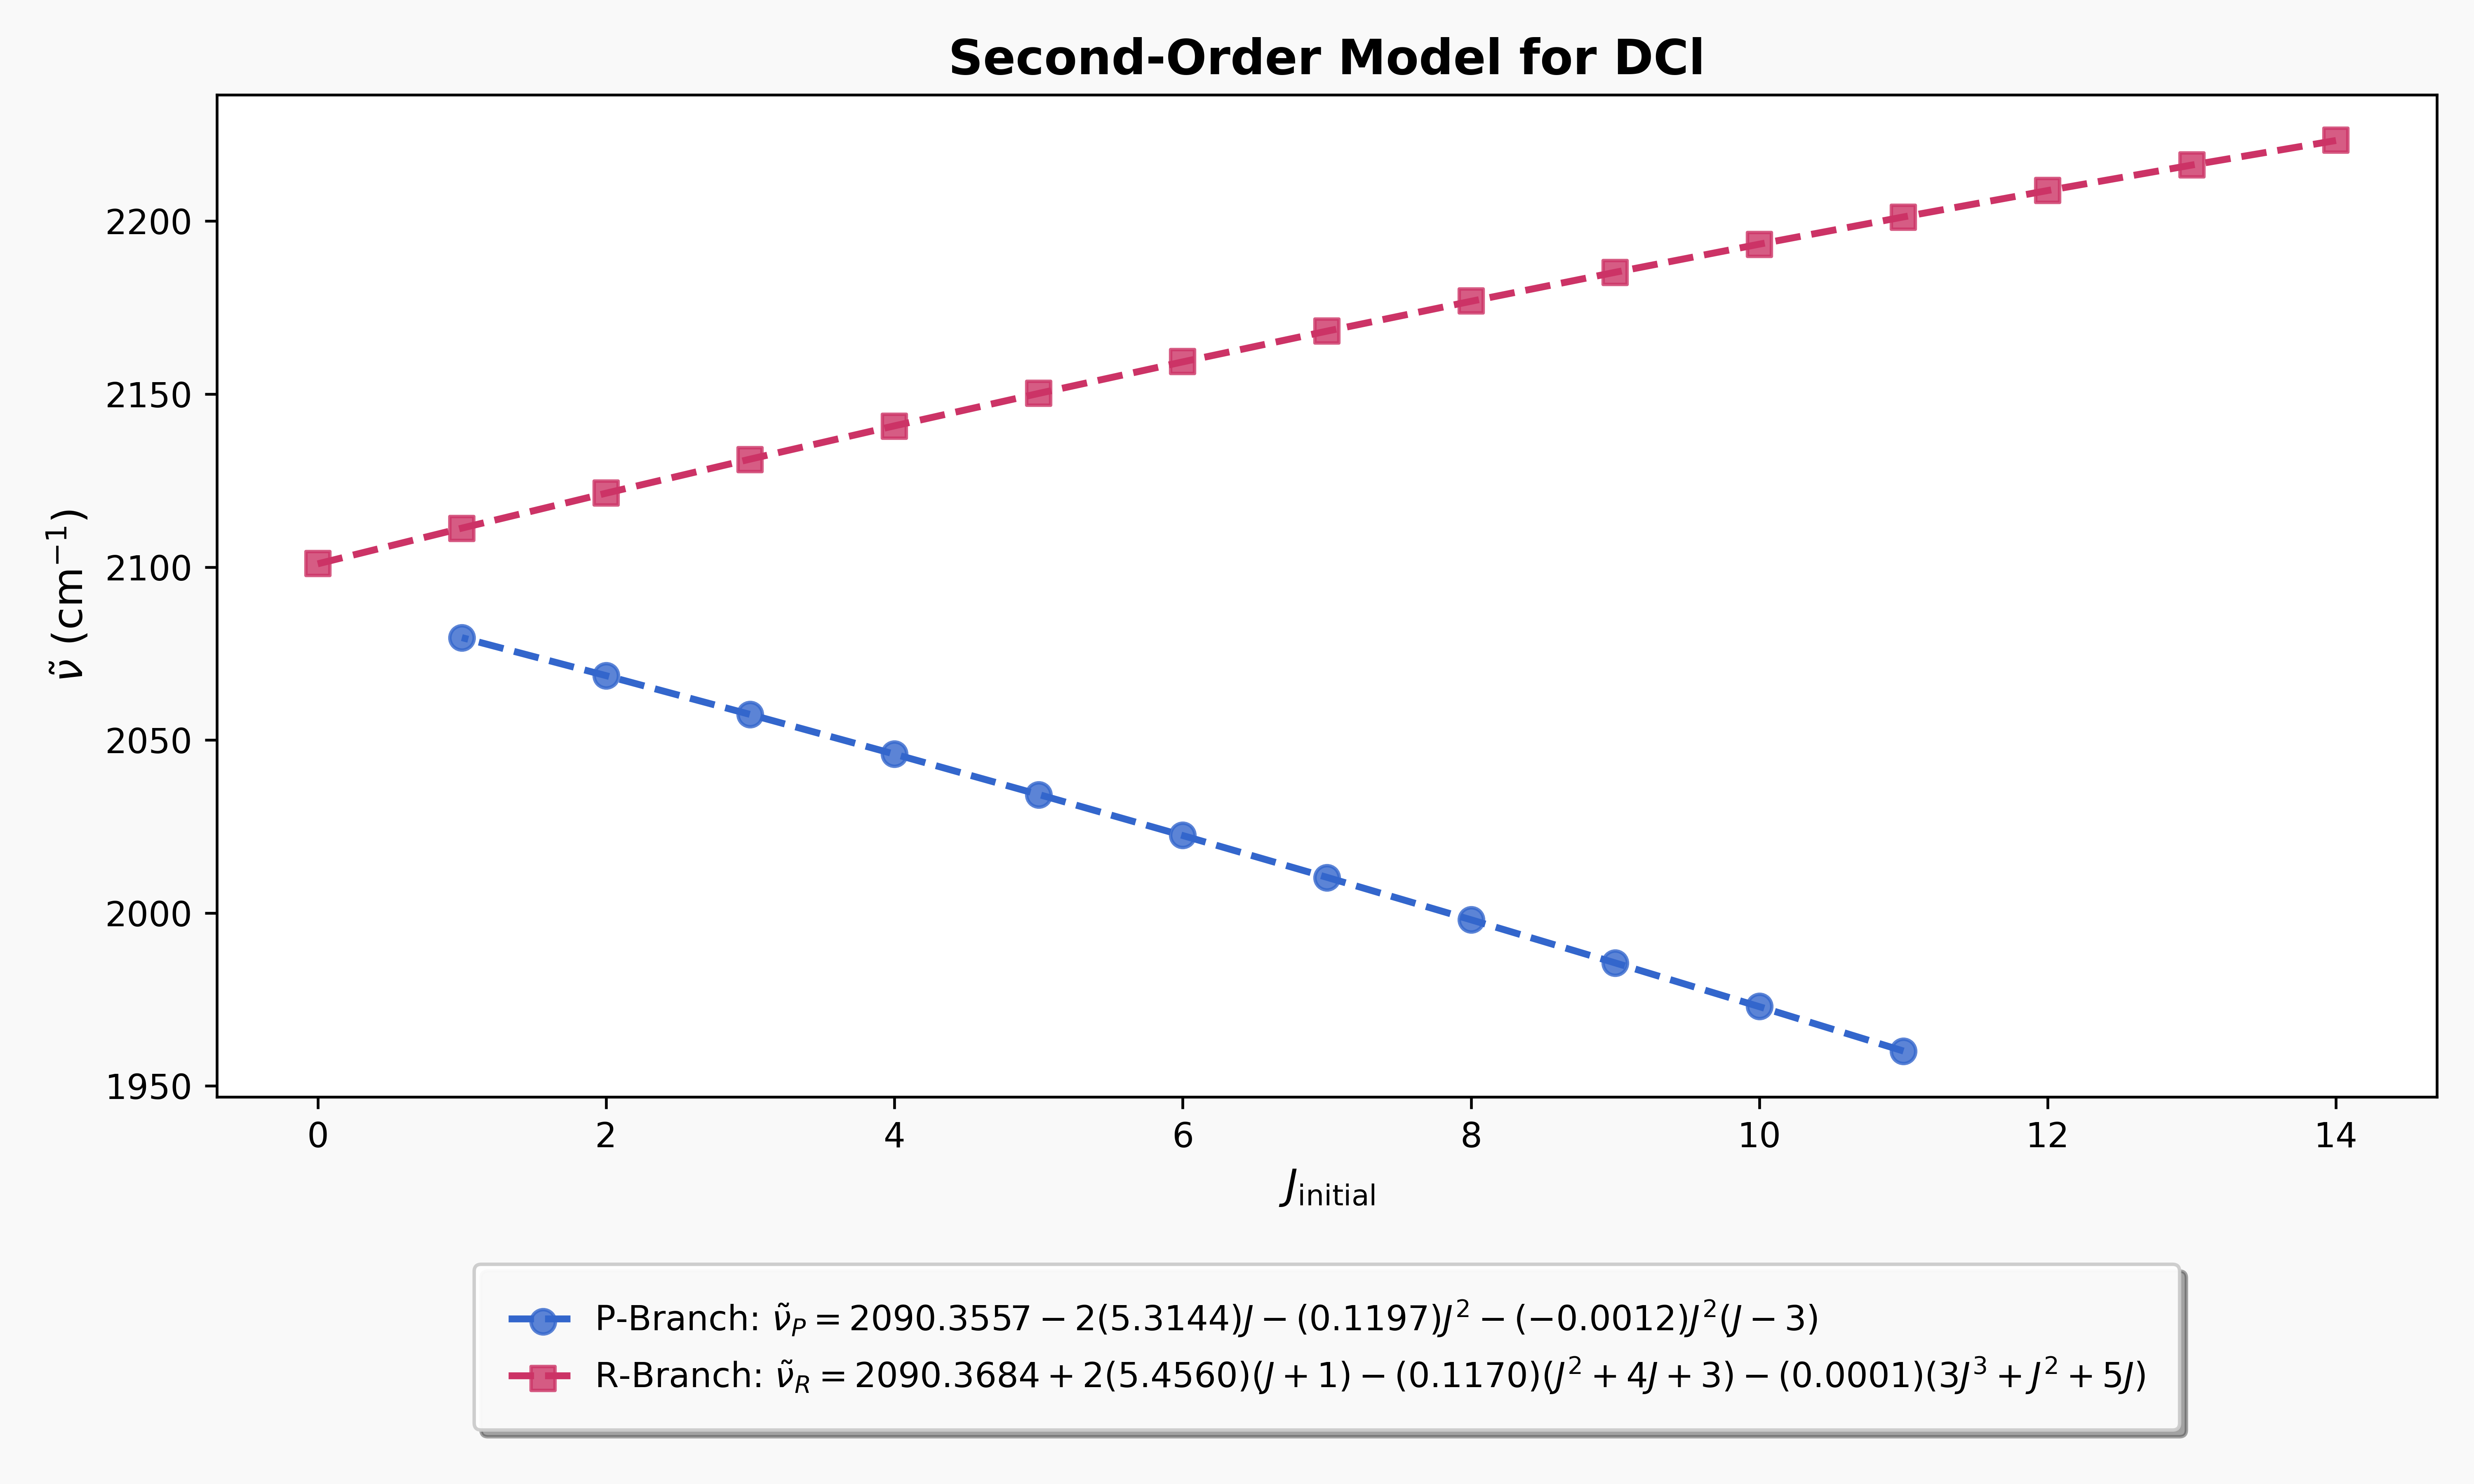
\includegraphics[width=\linewidth]{example-analysis/dcl-second-order-fit.png}
    \end{minipage}
\caption*{\mbox{}}
\begin{minipage}[t]{\textwidth}
        \centering
        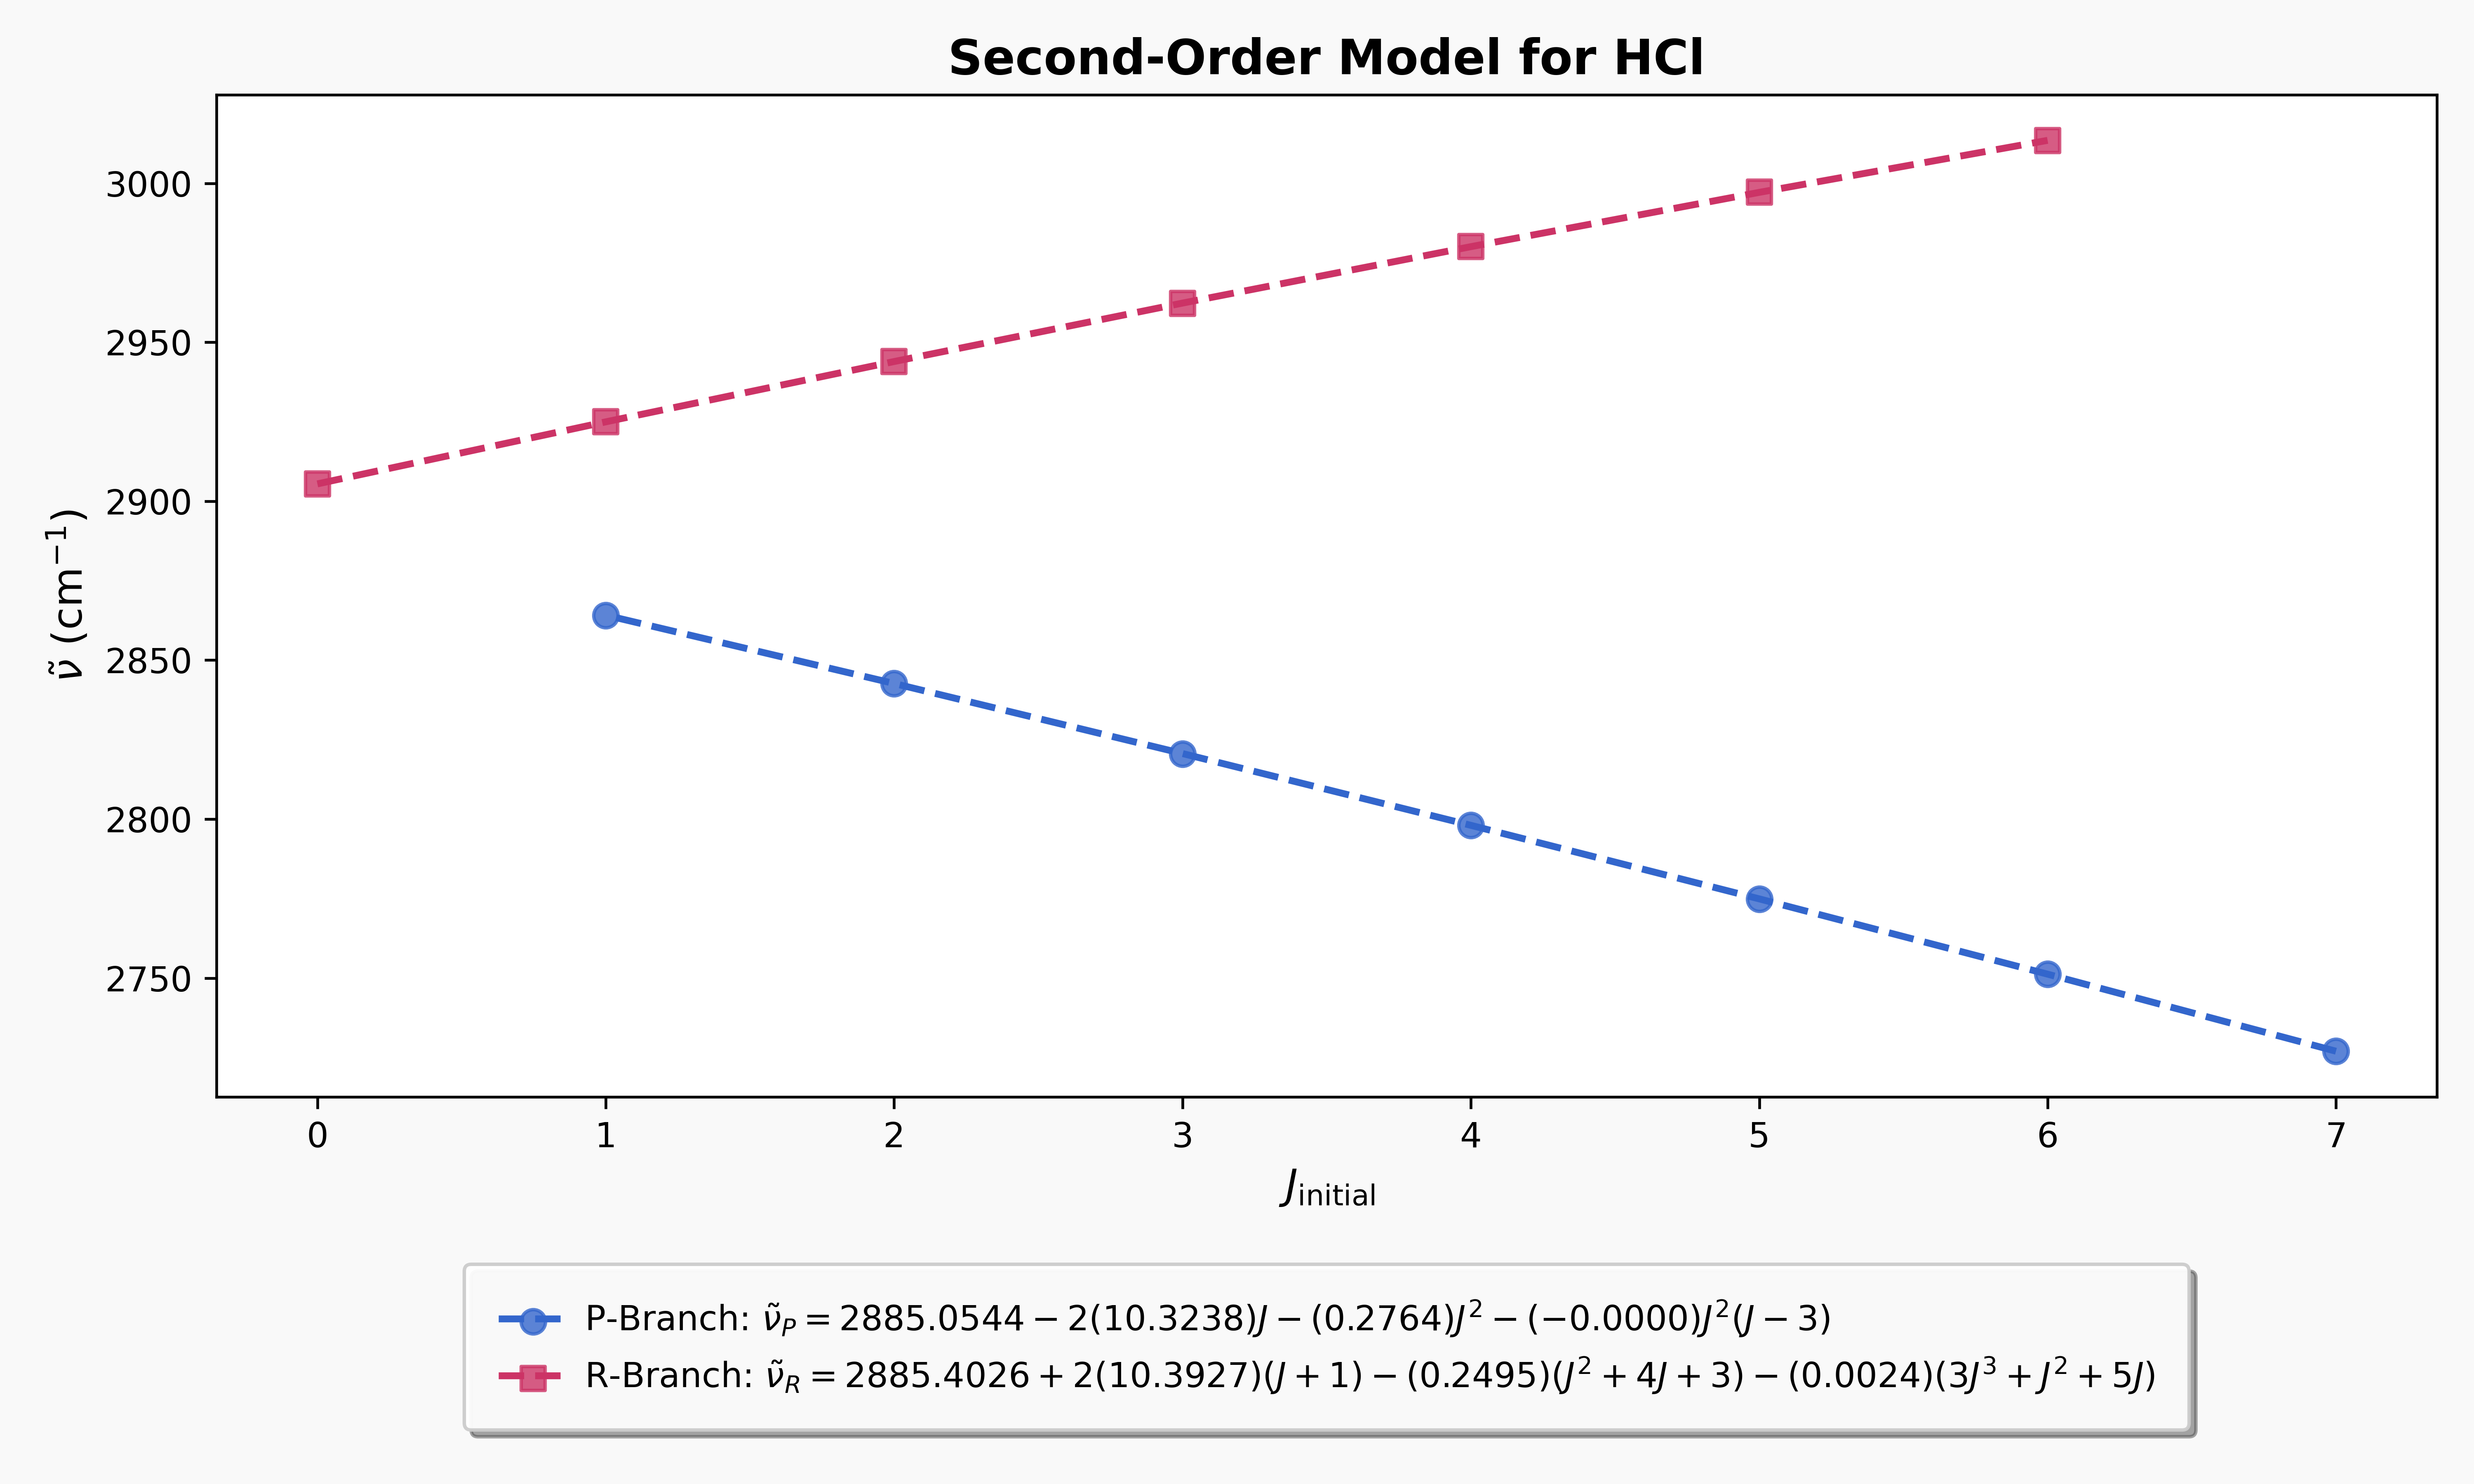
\includegraphics[width=\linewidth]{example-analysis/hcl-second-order-fit.png}
    \end{minipage}
\end{figure}
\begin{figure}[hbtp]
    ~\usesubsection{Background}
    The second order approximation is:
    \begin{align*}
        E_{2} &= h f_{0} \left(
            n + \frac{1}{2}
        \right) + hc BJ \left(J + 1\right)
        - h c \alpha \left(
            n + \frac{1}{2}
        \right)J \left(J + 1\right)
        - h c \delta J^2 \left(J + 1\right)
    \end{align*}
    The second order approximation assumes the diatomic molecule
    consists of two coupled systems: a simple harmonic oscillator
    (SHO) representing the vibrational energy, and a rigid rotator
    (RR) representing the rotational energy. In contrast with the 
    first order approximation, it takes into account the effects
    of centrifugal distortion caused by the rotation of the molecule. 
    The centrifugal force of the rotation of the molecule causes the 
    bond length, \(r_e\), to increase. Since the rotational constant,
    \(B\), is inversely proportional to the bond length, the centrifugal 
    distortion term, \(\delta\), corrects for this by lowering the overall 
    calculated energy. Since this term only concerns centrifugal distortion, it is
    only based w.r.t. the rotational quantum number, \(J\). Since rotational 
    energy contributes a relatively small amount to the overall energy 
    of the system, this corrective factor will be very small. 
    The peak in a rovib spectra is therefore the difference between sum of the change in vibrational energy and the change in rotational
    energy, and the sum of the coupling and centrifugal distortion terms. 
    ~\usesubsection{P-Branch Derivations}
    The second order energies for the P-Branch are given by
\begin{align*}
    \Delta E_{\delta, P} &= h c \delta \left(
        J - 1
        \right)^2 \left(
            J - 1 + 1
        \right) - h c \delta J^2 \left(
            J+1
        \right) \\
    &= h c \delta \left[
        \left(J-1\right)\left(J-1\right)
        \left(J\right) 
        - J^3 - J
        \right] \\
    &= h c \delta \left[
        J^3 - 3J^2
    \right] \\
    &= h c \delta J^2 \left(
        J - 3
    \right) \\
\end{align*}
    With the position of the peaks given by
    \begin{align*}
        \Delta E_{2, P} &= 
        \Delta E_{n} + \Delta E_{J, P}
        - \Delta E_{\alpha, P}
        - \Delta E_{\delta, P} \\
        \Delta E_{2, P}  &= 
        hf_{0} -hc\left(2BJ\right) - hc \alpha J \left(
            J - 2\left(n + 1\right)
        \right)
        - h c \delta J^2 \left(
            J - 3
        \right) \\
        \frac{\Delta E_{2, P}}{hc} 
        &= \frac{f_0}{c} - 2BJ - \alpha J^2
        - \delta J^2\left(J-3\right) \\
        \tilde{\nu}_{P} &= \tilde{\nu}_0
        - 2BJ - J^2 \left[
            \alpha + \delta\left(
                J-3
            \right)
        \right] \quad  \\
    \end{align*}
\end{figure}
\begin{figure}[hbtp]
    ~\usesubsection{R-Branch Derivations}
    The second order energies for the R-branch are given by
\begin{align*}
    \Delta E_{\delta, R} &=
    h c \delta \left[
        \left(J+1\right)^2
        \left(J+1+1\right) 
        - J^2\left(J+1\right)
    \right] \\
    &= hc \delta \left[
        3J^3 +J^2 + 5J
    \right] \\
    \end{align*}
    With the position of the peaks given by
    \begin{align*}
        \Delta E_{2, R} &=
        \Delta E_{n} + \Delta E_{J, R} 
        - \Delta E_{\alpha, R} 
        - \Delta E_{\delta, R} \\
        \frac{\Delta E_{2, R}}{hc} &= 
        \tilde{\nu}_0 + 2B\left(J+1\right)
        - \alpha\left[
            J\left(J+4\right) + 3
        \right] 
        -  hc \delta \left[
            3J^3 +J^2 + 5J
        \right] \\
\end{align*}
~\usesubsection{Fundamental Wavenumber}
After we perform a linear regression on the data for DBr, 
we get for the R-Branch \(
\tilde{\nu}_{R} = 1839.6647 + 2 \left(
    4.1103
\right) \left(
    J + 1
\right) - \left(
    0.0481
\right) \left(
    J^2 + 4J + 3
\right) - \left(
    0.0007
\right)\left(
    3 J^3 + J^2 + 5J
\right)
\), and for the P-branch \(
\tilde{\nu}_{P} = 1839.0768 - 2 \left(
    4.2050
\right)J - \left(
    0.0827
\right)J^2 + \left(
    0.0004
\right)J^2 \left(J - 3\right)
\). Calculating the average gives
\begin{align*}
    \tilde{\nu}_{0} &= \frac{\tilde{\nu}_{R} + \tilde{\nu}_P}{2} 
    = \frac{1839.6647 + 1839.0768}{2} 
    \approx 1839.3708 \mathrm{cm}^{-1} \\
    SD &= \sqrt{
        \frac{
            \left(
                1839.6647 - 1839.3708
            \right)^2
        + \left(
            1839.0768 - 1839.3708
        \right)^2
        }{2}
    }  \\
    \approx 0.293950 \mathrm{cm}^{-1} \\
    SE &= \frac{SD}{\sqrt{2}} \\
    &= \frac{0.293950}{\sqrt{2}} 
    &\approx 0.2079 \mathrm{cm}^{-1} \\
    \mathbf{\tilde{\nu}}_{0} &= \mathbf{
        \left(
            1839.3708 \pm 0.2079
        \right) cm^{-1}
    } \\
\end{align*}
\end{figure}
\begin{figure}[htbp]
    ~\usesubsection{Rotational Constant}
    \begin{align*}
        B &= \frac{B_{R} + B_{P}}{2} 
        = \frac{4.1103 + 4.2050}{2} 
        \approx 4.1576 \mathrm{cm}^{-1} \\
        SD &= \sqrt{
            \frac{
                \left(
                    4.2050 - 4.1576
                \right)^2
            + \left(
                4.1103 - 4.1576
            \right)^2
            }{2}
        }
        \approx 0.0473500 \mathrm{cm}^{-1} \\
        SE &= \frac{SD}{\sqrt{2}} 
        = \frac{0.0473500}{\sqrt{2}}
        \approx 0.0335 \mathrm{cm}^{-1} \\
        \mathbf{B} &= \mathbf{
            \left(
                4.1576 \pm 0.0335
            \right) cm^{-1}
        } \\
    \end{align*}
    ~\usesubsection{Rotational-Vibrational Coupling Constant}
    \begin{align*}
        \alpha &= \frac{\alpha_{R} + \alpha_{P}}{2} 
        = \frac{0.0481 + 0.0827}{2}
        \approx 0.0654 \mathrm{cm}^{-1} \\
        SD &= \sqrt{
            \frac{
                \left(
                    0.0481 - 0.0654
                \right)^2
            + \left(
                0.0827 - 0.0654
            \right)^2
            }{2}
        } \approx 0.0173 \mathrm{cm}^{-1} \\
        SE &= \frac{SD}{\sqrt{2}}
        = \frac{0.0173}{\sqrt{2}} 
        \approx 0.0122 \mathrm{cm}^{-1} \\
        \mathbf{\alpha} &\mathbf{= 
            \left(
                0.0654 \pm 0.0122
            \right) cm^{-1}
        } \\
    \end{align*}
    ~\usesubsection{Centrifugal Distortion Constant}
    \begin{align*}
        \delta &= \frac{\delta_{R} + \delta{P}}{2} 
        = \frac{0.0007 - 0.0004}{2}
        \approx 0.00015 \mathrm{cm}^{-1} \\
        SD &= \sqrt{
            \frac{
                \left(
                    0.0007 - 0.00015
                \right)^2
            + \left(
                -0.0004 - 0.00015
            \right)^2
            }{2}
        } \approx 0.00055 \mathrm{cm}^{-1} \\
        SE &= \frac{SD}{\sqrt{2}}
        = \frac{0.00055}{\sqrt{2}} 
        \approx 0.00039 \mathrm{cm}^{-1} \\
        \mathbf{\delta} &\mathbf{= 
            \left(
                0.00015 \pm 0.00039
            \right) cm^{-1}
        } \\    \end{align*}
\end{figure}
\begin{figure}[htbp]
    ~\usesubsection{Equilibrium Radius}    
    \begin{align*}
        r_{e, R} &= \sqrt{
            \frac{h}{8 \pi^2 c \mu_{\text{\scriptsize DBr}}  B_{R}}} \\
        &= \sqrt{
        \frac{0.0399031221 \mathring{A}^2 \cdot \nicefrac{\mathrm{amu}}{\mathrm{fs}}}{
        \left(
            8 \pi^2
        \right)    
        \left(
            2.99792458\times 10^{3}\nicefrac{\mathring{A}}{\mathrm{fs}}
        \right) \left(
            1.9646 \cdot \mathrm{amu}
        \right)
        \left(
            4.1103 \times 10^{-8} \mathring{A}^{-1}
        \right) 
        }}\\
        &\approx 1.449 \mathring{A} \\
        r_{e, P} &= \sqrt{
            \frac{h}{8 \pi^2 c \mu_{\text{\scriptsize DBr}}  B_{P}}} \\
        &= \sqrt{
        \frac{0.0399031221 \mathring{A}^2 \cdot \nicefrac{\mathrm{amu}}{\mathrm{fs}}}{
        \left(
            8 \pi^2
        \right)    
        \left(
            2.99792458\times 10^{3}\nicefrac{\mathring{A}}{\mathrm{fs}}
        \right) \left(
            1.9646 \cdot \mathrm{amu}
        \right)
        \left(
            4.2050 \times 10^{-8} \mathring{A}^{-1}
        \right) 
        }}\\
        &\approx 1.4285 \mathring{A} \\
        r_{e} &= \frac{ r_{e, R} + r_{e, P}}{2} \\
        &= \frac{1.449 + 1.4285}{2} \\
        &\approx 1.4367 \mathring{A} \\
        SD &= \sqrt{
            \frac{
                \left(
                    1.449 - 1.4367
                \right)^2
            + \left(
                1.4285 - 1.4367
            \right)^2
            }{2}
        } \\
        &\approx 0.0104530 \mathring{A} \\
        SE &= \frac{SD}{\sqrt{2}} \\
        &= \frac{0.0104530}{\sqrt{2}} \\
        & \approx 0.0074 \mathring{A} \\
        \mathbf{r_e} &= \mathbf{
            \left(
                1.4367 \pm 0.0074
            \right) \mathring{A}
        } \\
    \end{align*}
    ~\usesubsection{Moment of Inertia}
    The moment of inertia for the P-branch is \(
    I_{P} \approx 4.0089 \mathrm{amu} \cdot \mathring{A}^2
    \) and for the R-Branch \(
    I_{R} \approx 4.1014 \mathrm{amu} \cdot \mathring{A}^2
    \). This gives an average of \(
    \mathbf{\left(
        4.0551 \pm 0.0327
    \right) amu \cdot \mathring{A}^2}
    \)
    \end{figure}
\end{document}
